\documentclass[12pt, a4paper, twoside]{report}
\usepackage[utf8]{inputenc}
%%% Graphics
\usepackage{graphicx}
\graphicspath{{images/}}
%%% Page geometry
\usepackage[a4paper,width=150mm,top=25mm,bottom=30mm,bindingoffset=6mm]{geometry}
\usepackage{setspace}
%%% Page header
\usepackage{fancyhdr}
\pagestyle{fancy}
\usepackage[libertine,cmintegrals,cmbraces,vvarbb]{newtxmath}
%\usepackage[libertine,cmintegrals,cmbraces,vvarbb]{newtxmath, newtxtext}
%%% Units
\usepackage{siunitx}
\usepackage{titling}
\usepackage[round]{natbib}
%%% Math
\usepackage{amsmath}
\usepackage{bm}
%%% Color
\usepackage{xcolor}
%%% PDF include
\usepackage{pdfpages}
%%% Bibentries
\usepackage{bibentry}

% Appearance
%\usepackage{sectsty}
%\usepckage{helvet}
%\allsectionsfont{\sffamily}
%\allchaptersfont{\sffamily}

\title{Improving satellite measurements of clouds and precipitation using machine learning}
\author{Simon M. Pfreundschuh}
\date{\today}

%%%%%%%%%%%%%%%%%%%%%%%%%%%%%%%%%%%%%%%%%%%%%%%%%%%%%%%%%%%%%%%%%%%%%%%%%%%%%%%
% Customize header
%%%%%%%%%%%%%%%%%%%%%%%%%%%%%%%%%%%%%%%%%%%%%%%%%%%%%%%%%%%%%%%%%%%%%%%%%%%%%%%
\fancyhead{} % clear all header fields
\fancyhead[CO]{{\color{gray} \sc \footnotesize \leftmark}}
\fancyhead[CE]{{\color{gray} \sc \footnotesize \thetitle}}
\renewcommand{\headrulewidth}{0pt}
\fancyfoot{} % clear all footer fields
\fancyfoot[CE,CO]{\thepage}

\setlength{\headsep}{25pt}

\begin{document}

%%%%%%%%%%%%%%%%%%%%%%%%%%%%%%%%%%%%%%%%%%%%%%%%%%%%%%%%%%%%%%%%%%%%%%%%%%%%%%%
% Front matter
%%%%%%%%%%%%%%%%%%%%%%%%%%%%%%%%%%%%%%%%%%%%%%%%%%%%%%%%%%%%%%%%%%%%%%%%%%%%%%%
\pagenumbering{Roman} 

\begin{titlepage}
  \begin{center}

    {\sc%
      THESIS FOR THE DEGREE OF DOCTOR OF PHILOSOPHY 
    }

    \vspace*{5cm}
    \Large{\textbf{\thetitle}}
    \normalsize

    
    \vspace{1.0cm}

    \theauthor

    \vfill
    
    \vspace{5cm}

    {\setstretch{1.5}
      Department of Earth, Space and Environment \\
      {\sc CHALMERS UNIVERSITY OF TECHNOLOGY}\\
      Gothenburg, Sweden, 2022 \\
    }


    
    
  \end{center}
\end{titlepage}

\thispagestyle{plain}
\vspace*{5cm}

\noindent\textbf{\thetitle}\\[0.2cm]
%
\nodindent \theauthor \\
ISBN 978-91-7905-657-5\\[0.5cm]

\noindent \copyright \ {\sc SIMON M. PFREUNDSCHUH} \\[0.5cm]



\noindent Doktorsavhandlingar vid Chalmers tekniska högskola \\
Ny serie nr 5123  \\
ISSN 0346-718X  \\[0.5cm]

\noindent Department of Space, Earth and Environment \\
Chalmers University of Technology  \\
SE-412 96 Gothenburg  \\
Sweden 
Telephone + 46 (0)31-772 1000  \\[2cm]

%\vfill \noindent Cover:  \\
%\noindent [en förklarande bildtext till eventuell omslagsbild, med sidhänvisning till utförligare 
%  information i uppsatsen / an explaining legend if there is an illustration on the cover together 
%  with a page number to read more] \\[0.5cm]
\noindent Chalmers digitaltryck  \\
\noindent Gothenburg, Sweden 2022 

\clearpage

\thispagestyle{plain}
\begin{center}
  {\large \textbf{\thetitle}}
  
  \vspace{0.4cm}
  
  \vspace{0.4cm}
  {\sc \theauthor}
  
  \vspace{0.9cm}
  \textbf{Abstract}
\end{center}

\bibliographystyle{plainnat}
\nobibliography*

\clearpage

\chapter*{List of publications}

\section*{Appended articles}

This thesis is based on the work contained in the following papers:

\begin{description}
\item[\textbf{Paper 1:}] \bibentry{pfreundschuh18}
\item[\textbf{Paper 2:}] \bibentry{pfreundschuh22a}
\item[\textbf{Paper 3:}] \bibentry{pfreundschuh22d}
\item[\textbf{Paper 4:}] \bibentry{pfreundschuh22b}
\item[\textbf{Paper 5:}] \bibentry{kaur21}
\end{description}

\section*{Other relevant publications}

\begin{enumerate}
\item \bibentry{kaur22}
\item \bibentry{pfreundschuh22c}
\item \bibentry{pfreundschuh20}
\item \bibentry{ekelund20}
\item \bibentry{hagen20}
\item \bibentry{duncan19}
\item \bibentry{duncan19b}
\end{enumerate}

\tableofcontents
\clearpage

%%%%%%%%%%%%%%%%%%%%%%%%%%%%%%%%%%%%%%%%%%%%%%%%%%%%%%%%%%%%%%%%%%%%%%%%%%%%%%%
% Kappa
%%%%%%%%%%%%%%%%%%%%%%%%%%%%%%%%%%%%%%%%%%%%%%%%%%%%%%%%%%%%%%%%%%%%%%%%%%%%%%%
\pagenumbering{arabic} 

\part{Introductory chapters}

\chapter{Introduction}

Earth observation satellites play an essential role in many scientific and
meteorological applications. Their unique ability to provide frequent
observations of large parts of the globe allows meteorologists to predict the
weather and scientists to study the Earth and its atmosphere. Weather
predictions and the monitoring of the climate are of considerable
societal and economic value, a value that is likely to increase as the 
Earth continues to warm.

Observations from these satellites consist of measurements of electromagnetic
radiation, which is either reflected or emitted from the Earth and its
atmosphere. An example of such measurements is given in
Fig.~\ref{fig:introduction:water_vapor}. Besides demonstrating its delicate
beauty, this image of infrared radiation emitted from a low-pressure system over
the Mediterranean sea contains valuable information about the physical state of
the atmosphere. The colors in the image represent the intensity of the measured
radiation from strong to weak using bright to dark colors. At this specific
wavelength, the measured radiation stems from water vapor and clouds in the
atmosphere. Dry air is less opaque and allows the satellite to sense
radiation from lower down in the atmosphere. Since the temperatures in the lower
atmosphere increase with decreasing height, the radiation in these regions is
more intense. Bright colors thus identify regions of relatively dry air. Moist
air, which is more opaque, emits radiation from higher up in the atmosphere
where temperatures are lower and thus produces the moderate intensities that are visible in the
image. The lowest intensities stem from high clouds, which are fully opaque and
thus emit radiation at high altitudes and low atmospheric temperatures.

\begin{figure}[h!]
\centering
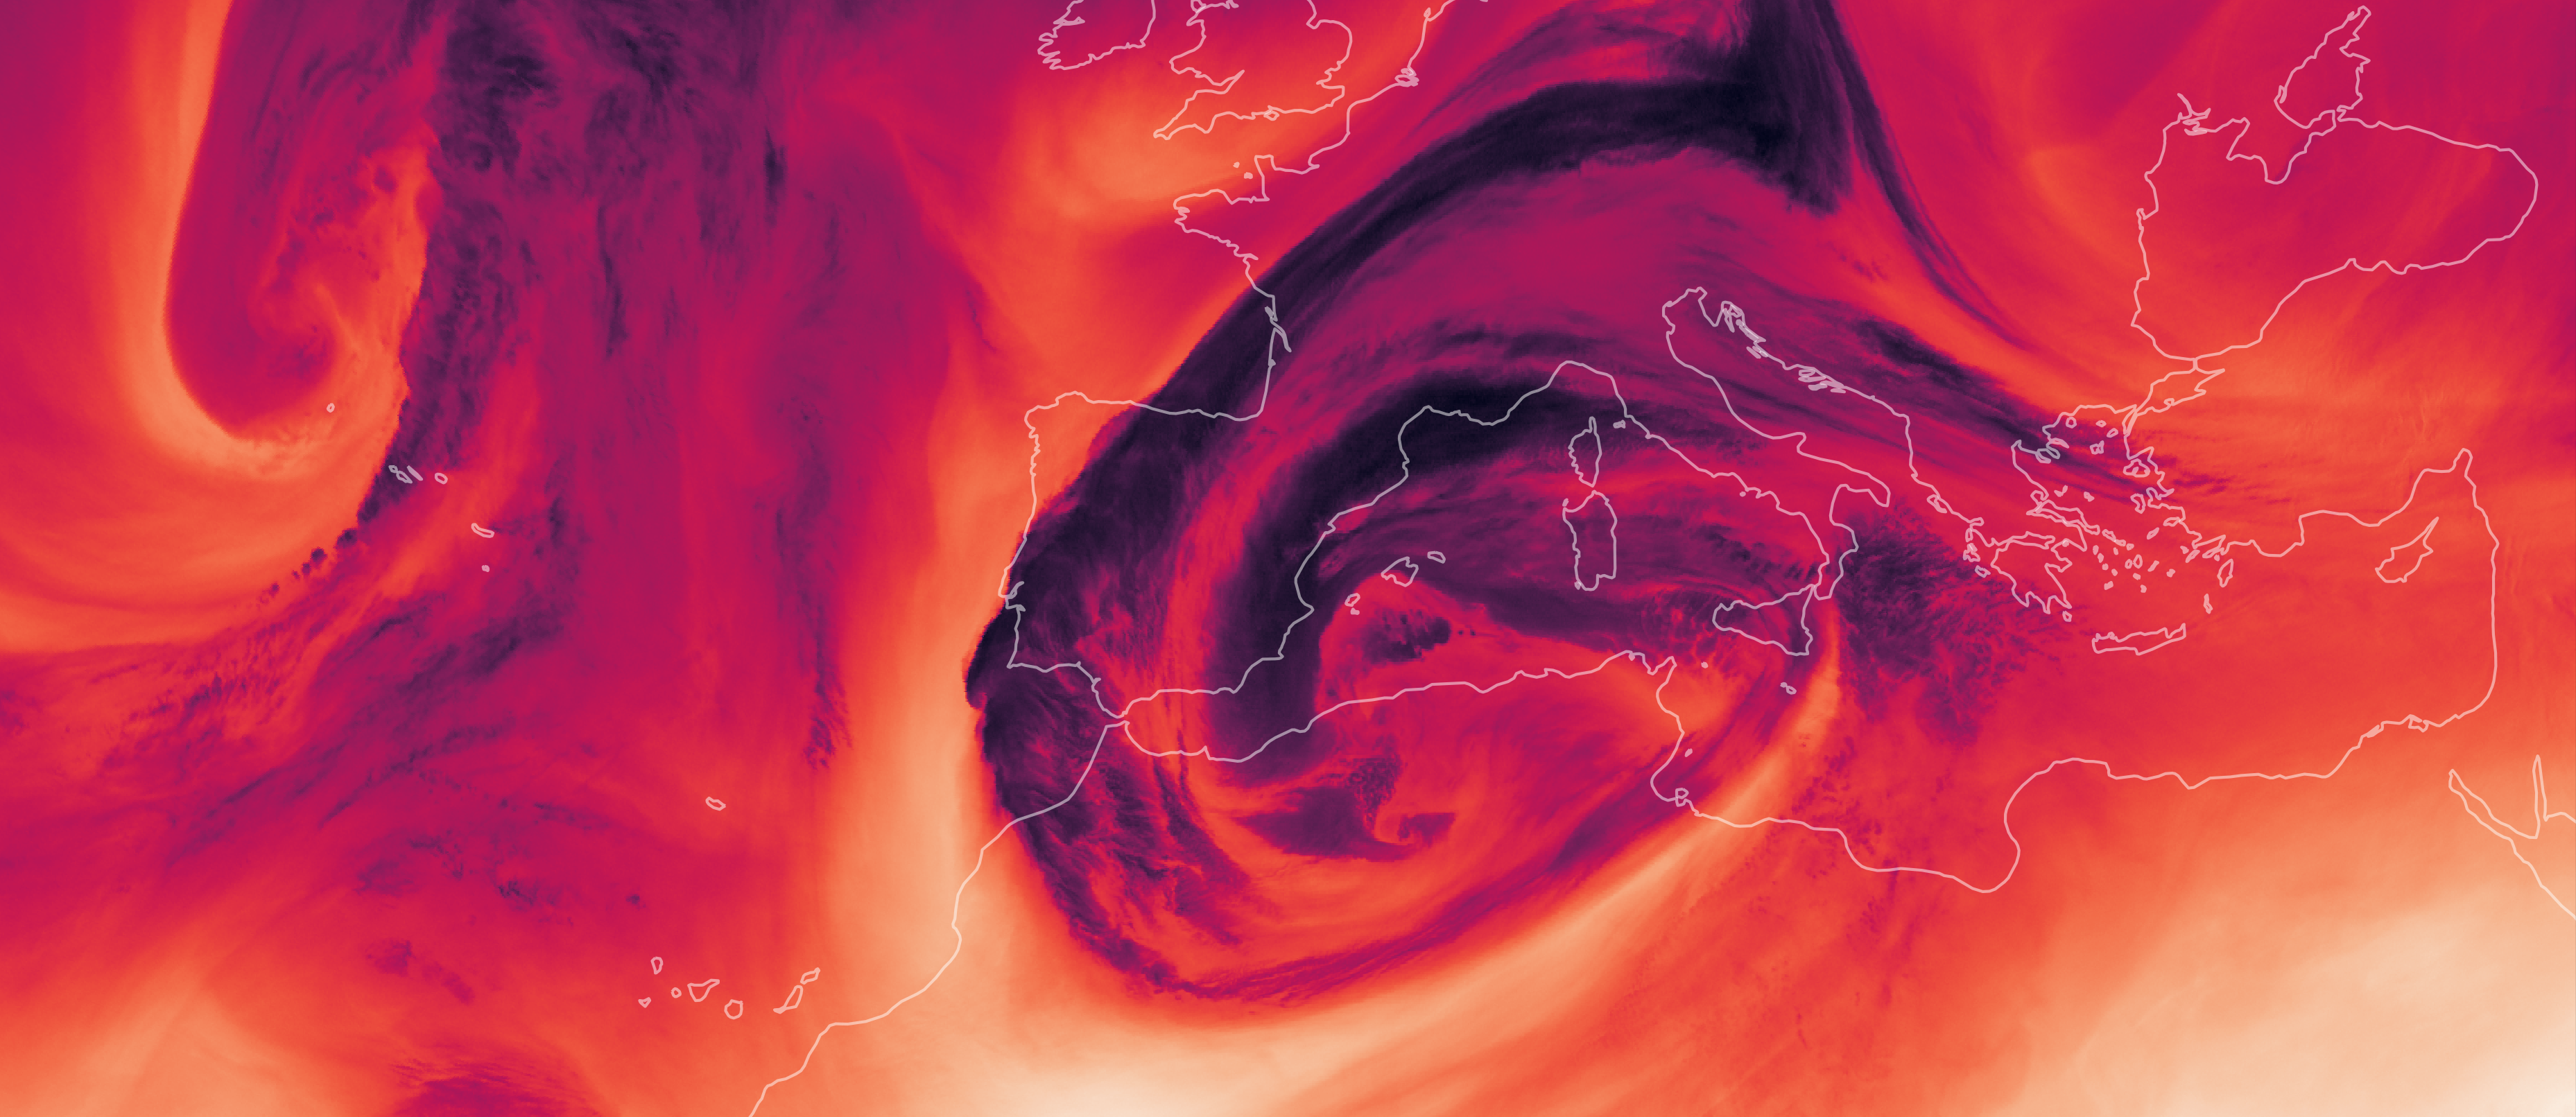
\includegraphics[width=\textwidth]{water_vapor}
\caption{Water vapor (white to red) and high clouds (purple to black) over the
Mediterranean as observed by the Spinning Enhanced Visible and Infrared
Imager at a wavelength of $\SI{6.2}{\micro \meter}$.}
\label{fig:introduction:water_vapor}
\end{figure}

This example illustrates that an understanding of the processes that generate
the infrared radiation observed by a satellite allows an observer to infer
moisture content and the presence of high clouds in the atmosphere.
Formulated more generally: If a component of the atmosphere interacts
sufficiently strongly with radiation, it generates an electromagnetic signal
that can be measured using a suitable sensor. By inverting the component's
interaction with the observed radiation, these measurements can be used to infer
the properties defining the interaction. This inversion process is
called \textit{the retrieval} and is required to relate satellite observations
to the physical state of the atmosphere.

The subject of this thesis is the retrieval of
properties of clouds and precipitation from satellite observations. These measurements are difficult
due to the high variability in the appearance and composition of clouds and,
secondly, the complexity of their interaction with radiation. At the
same time, the important role that clouds and precipitation play in the weather
and climate system makes these measurements highly relevant for science and
society.

To set the scene for the discussion of satellite observations and retrieval
techniques in the subsequent chapters, this introduction aims to provide an
overview of the relevance of observing and measuring clouds and precipitation
from space. Beginning with the societal significance of water, the discussion
will move on to the scientific relevance of observing water as it moves through
the atmosphere.



\section{Water as resource}

Water is essential to life on Earth. It is the bloodstream of the biosphere
\citep{falkenmark04} and a fundamental resource to all forms of human
societies. The largest part of human freshwater consumption from lakes, rivers
or ground water, so called \textit{blue water} consumption, is used to irrigate
crops, while domestic and industrial use play minor roles. Blue water
consumption is distinguished from \textit{green water} consumption, which refers
to the part of precipitation which is involved in the photosynthesis process.
Although rarely considered in consumption inventories, green water plays an
important role in providing water for rain-fed agriculture, which accounts for
$\SI{60}{\percent}$ to $\SI{70}{\percent}$ of the global food production, as
well as in the sustaining of terrestrial ecosystems \citep{falkenmark04}.

Humans depend on water for food production both through irrigation from
blue water flows and the provision of soil moisture by green water flows.
Achieving food security has been recognized by the United Nations (UN) as a
sustainable development goal (SDG, \citeauthor{sdg}, \citeyear{sdg}). The large
contribution of food production to overall water consumption poses a challenge
to the management of water resources. Diverting more blue or green water flows
for the production of food reduces the amount of water that is available to
sustain terrestrial and aquatic ecosystems. There is thus direct potential for
conflict between SDG number two to end hunger and the SDGs 14 and 15 to sustain
terrestrial and aquatic ecosystems.

At the same time, water requirements for the production of energy are expected
to increase as fossil fuels are increasingly sourced from unconventional
deposits, such as shale oil and gas, whose extraction consumes substantial
amounts of water \citep{rosa18}. This is accompanied by a projected increase in
hydropower \citep{zarfl15} and the use of biofuels, both of which are reliant on
and affect freshwater supplies. This emerging competition in water uses is
recognized as the \textit{food-energy-water} nexus \citep{dodorico18}.




% Also here satellite observations that allow
%the monitoring of water resource are an important tool for the effective
%management of droughts \citep{boyd13}.

%Water consumption is typically categorized into two classes: blue and
%green water consumption. Blue water consumption refers to 
%
%The consumption of water is typically categorized as blue water consumption,
%which refers to the extraction of surface water from rivers or ground water, and
%green water consumption, which refe to rain water consumed directly, for example
%to grow crops. Of the global blue water consumption, agricultural activity
%constitutes the largest part followed by industrial activity and domestic use
%\citep{falkenmark04}. Agriculture, however, also consumes large amounts of
%green water as $60$ to $\SI{70}{\percent}$ of the world's  food is produced on
%rainfed land.
%
%Water also plays an important role as source of energy. In the year 2020, energy
%produced from hydroelectric plants constituted one sixth of the global energy
%production \citep{eia21} and it can be expected that this portion will increase
%with the required decarbonization of the energy sector.


\section{The hydrological cycle}


Sustainable human water consumption depends on the replenishment of the sources
from which water is obtained. Freshwater over land exists in the form of
glaciers, ice sheets, lakes and reservoirs, snowpacks, wetlands, rivers, and a small part contained in the biomass. Water also exists within the land
surface in the form of soil moisture, permafrost, and groundwater. The largest
part of the water that is available on the surface of the Earth is stored in the
oceans. Only a very small part is stored in the atmosphere. Most of that is in
the form of water vapor, and only a minor fraction is contained in clouds in the
form of liquid droplets or ice crystals \citep{abbott19}.

Despite containing only a tiny fraction of the global water reserves at any
given moment, the atmosphere is responsible for essentially all of the water
transport from oceans to land. An illustration of the atmospheric branch of the
hydrological cycle is provided in Fig.~\ref{fig:introduction:water_cycle}. The
largest flux in this part of the hydrological cylce is the influx of water vapor
by evaporation from the ocean surface. Most of the water vapor that evaporates
over the ocean never reaches the land but instead returns to it in the form of
precipitation. Only about $\SI{10}{\percent}$ of the evaporation over oceans is
transported to land, where it may form precipitation to replenish the water
storages from which it is available for human consumption. A significant part of
that precipitation evaporates again, allowing it to take part in the formation
of precipitation further inland.


\begin{figure}
\centering
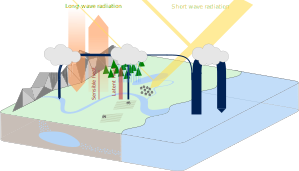
\includegraphics[width=0.8\textwidth]{water_cycle_energy}
\caption{
Illustration of the atmospheric branch of the hydrological cycle. Dark blue
arrows show the flow of water into, within and out of the atmosphere. Their
width approximately represents the extent of these fluxes. The
semi-transparent arrows in orange, yellow and red show the energy fluxes in the
Earth system, which are directly coupled to the hydrological cycle through
the radiative effects of water vapor, clouds and the release of latent heat.}
\label{fig:introduction:water_cycle}
\end{figure}

On the scale of river basins, the inflow of water through the atmosphere is the
only sustainable source of freshwater \citep{falkenmark04}. Given the competing
water requirements for the production of food and energy, as well as ensuring
access to clean water and  sustaining of ecosystems, it is clear that water
management is required to avoid conflicts, minimize human suffering and reduce
ecological damage. This management has to rely on the monitoring and modeling of
the hydrological cycle. Since water fluxes within the hydrological cycle are
highly variable in space and time and occur across continental scales, satellite
observations are currently the only way through which continuous monitoring of
the hydrological cycle can be realized.

\section{Weather and climate}


Water in its various forms is a fundamental component of the Earth's weather
\citep{stevens13}.
When it evaporates, it takes up energy from the environment. This energy, the
\textit{latent heat}, is released when the air cools and the water vapor condensates. The
release of latent heat acts as fuel for the development of vigorous convective
storms. The water that is released by those storms in the form of precipitation
can cause flooding and landslides.

The ability to predict the weather has considerable value for society,
especially for high-impact events involving extreme wind speeds and
precipitation. The availability of satellite observations has played an
important role in the steady improvement of weather forecasts that occurred
during the last three decades
\citep{bauer15}. Weather forecasting systems use satellite data to
determine the best estimate of the current state of the atmosphere, which is then
evolved into the future to predict the weather. While advanced forecasting
systems ingest satellite observations directly and are thus not dependent on
satellite retrievals \citep{bauer10}, some systems use retrieved cloud
properties for the initialization of short-range forecasts
\citep{dehaan14, benjamin21}. Besides that, retrievals of precipitation and
cloud properties are used by weather forecasters to gain situational awareness
and assess potential weather hazards.

%Despite the progress of the last decades, weather forecasts still struggle to
%produce accurate forecasts for specific meteorological contexts
%\citep{schafler18}. In many of those, the misrepresentation of the
%interaction of latent heat release through condensation and the large scale
%dynamics of the atmosphere were found \citep{rodwell13} to play a role.
%Improving the forecasts requires improving the representation of these processes
%in the model, which is where satellite-derived measurements of precipitation and
%clouds can help researchers better understand them.

At the same time, water also has a pivotal role in the climate system. As
illustrated in Fig.~\ref{fig:introduction:water_cycle}, it is coupled to the
Earth's energy budget through multiple processes. Water vapor is the most potent
greenhouse gas and thus contributes strongly to the retention of radiative
energy emitted from the Earth's surface. In the form of clouds, water both cools
the Earth system through the reflection of solar radiation and warms it through
the absorption of upwelling longwave radiation. Although the global effect of
clouds is a pronounced cooling, the effect varies regionally and with the
properties of the clouds. Evaporation, transpiration, and convection are
important for the transfer of heat from the Earth's surface to the atmosphere.
Since, on average, evaporation and transpiration have to be balanced by
precipitation, the energy budget of the Earth is directly linked to
precipitation \citep{trenberth09}.

Instead of a passive tracer of atmospheric dynamics, water must thus be
understood as an active component of both the weather and the climate system
linking these systems to the hydrological cycle. Because of the global
extent and complex nature of these systems, satellite observations of the
hydrological cycle are essential for climate science and meteorology.


\section{A warmer planet}

As a consequence of anthropogenic emissions of carbon dioxide, the Earth's
 climate is warming. As the Earth system adapts to the increased radiative
 forcing from greenhouse gases, its climate changes. These changes are not
 uniform but exhibit significant regional variability. Reliable regional
 predictions of the future climate are thus required to help societies adapt to
 them. However, the current understanding, as well as the ability to predict
 changes at regional scales, remains limited.

The hydrological cycle is changing together with the climate. Because of the
ability of warmer air to hold more water, water vapor concentrations are
increasing. An increase in evaporative demand is expected to lead to more frequent
and severe droughts. At the same time, global precipitation is expected to
increase. Extreme precipitation events are strengthening and becoming more
frequent. At the scales of individual precipitation systems, precipitation
increases with the capacity of warmer air to carry water vapor. Globally,
however, evapotranspiration and thus also precipitation are constrained by the
Earth's energy budget, which limits increases in global precipitation to a lower
rate than that of individual storms \citep{collins13}. In addition to that,
changes in the general circulation will modify the global distribution of
precipitation.

As part of the hydrological cycle, clouds will change with the climate. Since
clouds reflect incoming solar radiation and  absorb outgoing long-wave
radiation, these changes act as a feedback on the Earth's energy budget and
will thus influence the response of the climate system to increased carbon dioxide
concentrations. Whether an individual cloud exerts  net warming or cooling
 on the climate system depends on its properties such as altitude,
 composition, and  location. The representation of clouds remains a
challenge for climate models and uncertainties in cloud feedbacks
remain the primary source of uncertainty in predictions of the climate response
to increased carbon dioxide concentrations in the atmosphere \citep{zelinka20}.

The understanding of climate change has progressed immensely during the last
decade but remains insufficient to make confident predictions at regional
scales. Such predictions are necessary for successful climate change adaptation.
Satellite observations are essential for improving and validating climate models
and monitoring changes in the climate system, making them a crucial
guide for the passage into an uncertain, warmer future.

\section{Why satellites?}

Considering the importance of rain for a large range of human activities, it is
not surprising that humans have been measuring precipitation and trying to
improve their understanding of the weather system. The most direct and arguably
intuitive way to measure precipitation is through the use of \textit{rain
gauges}. A rain gauge consists of a cavity that captures rain and from which the
accumulated precipitation can be measured. First records of gauge measurements
of rain date back to as long as 400 years BC \citep{strangeways2000}. Today,
gauge measurements are available from most populated regions across the globe.
However, their density varies from country to country and is oftentimes tied to
the local population density.

the main disadvantage of rain gauges is the highly localized character of their
measurements, which limits their ability to accurately capture the spatial
structure of precipitation on short time scales. moreover, because these
measurements are performed by a large number of public and private entities
across the globe, not all of them are easily accessible to scientists.
effectively, only $\si{1}{\percent}$ of the surface of the earth is estimated to
be within a distance of $\si{5}{\kilo \meter}$ from the nearest gauge
measurement \citep{kidd17}.

Ground-based radars are another important technique for measuring precipitation
over land. These radars send out beams of radiation, which are reflected by rain
and snow. Precipitation within a radius of several hundreds of kilometers can be
detected by measuring the amount of radiation that is reflected back to the
radar. Ground-based radars are important for the real-time monitoring of
precipitation over land. However, due to their high installation and maintenance
costs, their spatial availability is irregular and typically follows the local
population density. In addition to that, the availability and accuracy of radar
measurements may be hampered by complex terrain as well as the distance from the
radar location, which limits the utility of these observations for
climatological applications.

The relevance of clouds and precipitation for the hydrological cycle has been
known since before the times of Aristotle \citep{frisinger72}. Nonetheless, the
systematic study of clouds has long remained a secondary focus of
meteorology, and it took until the 1970s before the importance of interactions
between clouds, weather, and climate put them at the forefront of atmospheric and
climate research \citep{stephens03}. Traditionally, cloud observations were
conducted as parts of routine meteorological observations performed on land and
ships \citep{hughes84}. However, these observations were primarily qualitative,
indicating only the presence of clouds, their type and an  approximate
height.

The principal drawback of the measurement techniques discussed above is their
limited and irregular spatial coverage, which reduces their suitability for
monitoring the global weather and climate. In contrast to that, satellites have
the ability to provide observations across the globe at high temporal
resolutions. Therefore, they ideally complement ground-based measurements
and have become an essential source of information for a wide range of
scientific, economic and societal activities.



\chapter{Atmospheric radiative transfer}

This chapter now turns to the physical principles that enable satellites to
sense clouds and precipitation from space. The remote sensing of any atmospheric
quantity is based on its interaction with electromagnetic radiation. The
measured radiation can be used to infer physical properties of atmospheric
quantities by inverting the interaction between radiation and the atmosphere.
Doing so, requires a quantitative model of the propagation of radiation through
the atmosphere. Such a model is provided by the physical theory of radiative
transfer.

Since radiative transfer theory is fundamental to atmospheric remote sensing ,
this section provides an introduction to radiative transfer in the atmosphere.
The focus is put on the interaction of radiation with hydrometeors. This
presentation is mostly based on the more comprehensive texts by Mishchenko et
al. (2002), Thomas and Stamnes (2002), and Wallace and Hobbs (2006).


\section{Radiative transfer theory}

Radiative transfer theory describes the propagation of electromagnetic radiation
through a medium. It provides simplified model of the electromagnetic and
quantum mechanical interactions of a perfectly monochromatic beam of light.
Electromagnetic sensors measure the mean total energy that is transferred by
electromagnetic radiation as well the correlations between the components of the
beam's electric field, which define the beam's \textit{polarization state}. The
radiation measured by a sensor at position $\bm{r}$ pointing in direction
$\bm{-n}$ is fully described by the four dimensional stokes vector
\begin{align}
  \bm{I}(\bm{r}, \bm{n}) &= \left [ \begin{array}{c}
    I \\
    Q \\
    U \\
    V \\
    \end{array} \right ]
\end{align}

The components $I, Q, U$ and $V$ are called the stokes parameters and have the
unit of monochromatic energy flux. The stokes vector fully describes the state
of a monochromatic beam of radiation to the extent that it can be measured by an
electromagnetic sensor. Thus any electromagnetic measurement observation from
knowledge of the stokes vector at the position of the sensor. Radiative transfer
theory describes how the stokes vector changes as it propagates through a medium.

\subsection{Interactions with matter}

Radiative transfer theory distinguishes three fundamental processes through
which matter interacts which radiation. These are (1) the emission of
electromagnetic radiation, (2) its absorption and (3) scattering.

\subsubsection{Emission}

At temperatures above absolute zero, all matter emits radiation through the
process of thermal emission. Thermal emission occurs when matter transitions
from a quantum mechanical state of higher energy to one of lower energy which
causes the excess energy to be emitted in the form of radiation. The amount of
radiation of a given frequency $\nu$ emitted by a body depends on its
temperature and material. It is typically modeled using a material-dependent
emissivity vector $\vec{e}$, which relates the emission of the material to that
of an ideal black body, i. e. a material that absorbs all incoming radiation:
 \begin{align}
   \label{eq:emissivity}
   \vec{I} &= (\vec{e} \cdot ds) B(T, \nu)
 \end{align}
 Here $B(T, \nu)$ is the radiation emitted by a black body at temperature $T$
 and frequency $\nu$, which is described by Planck's law
 \begin{align}
   B(T, \nu) &= \frac{2 \nu^2}{c^2}\frac{h\nu}{e^{\frac{h\nu}{k T}} - 1},
 \end{align}
 with $c$ is the speed of light in vacuum, $h$  the Planck constant and $k$
 the Boltzmann constant.

The emissivity vector defined above is a differential quantity that describes
emission from a volume element along an infinitesimal step along the propagation
path. This means that in order to obtain the emission from a finite volume, the
emission must be integrated along the propagation path. For a material that is
opaque, there is no need to integrate over the full volume, since only its
surface will contribute to the observed emission. The emissivity of a surface
can be described using an emissivity vector $\vec{e}$ in the same way as for
emission from a volume, with the difference that its components are unitless
and integration over the propagation path is not required.

\subsubsection{Absorption}

Absorption refers to the process of radiation being converted into internal
energy of the matter it interacts with. Mathematically, this process is
described by the absorption vector $\vec{\alpha}$, defined as the fraction of
the incoming radiation that is absorbed along an infinitesimal distance $ds$
along the propagation path:
\begin{align}
\vec{I}_\text{absorbed} &= (\vec{\alpha} \cdot\ ds) \odot \vec{I}
\end{align}
Here $\odot$ denotes the element-wise product of the absorption vector and
the Stokes vector $\vec{I}$ of the incoming radiation. Absorption may be
understood as the inverse process of thermal emission. Formally, this is
expressed by Kirhoff's  law of radiation
\begin{align}
  \vec{\alpha} &= \vec{\epsilon},
\end{align}
which states that the absorption vector is identical to the emissivity vector
defined in Eq.~\ref{eq:emissivity}. This law is applicable to all matter in the
atmosphere given that it is in a state of local thermal equilibrium (LTE). LTE
occurs when the density of matter is sufficiently high so that the population
rates of energy states above the ground state are determined by thermal
collisions rather than the absorption of radiation. This decouples the emission
of radiation from the radiation field itself, allowing the simplified treatment
of matter as thermal emitters with the emission rates independent of the
radiation field. LTE is a valid assumption for radiative transfer in the
troposphere.

\subsubsection{Scattering}

Scattering describes the effect of inhomogeneities in the dielectric properties
of the medium on the propagation of the beam. When a plane-parallel
electromagnetic wave encounters such inhomogeneities, it is scattered in all
directions. Since parts of the energy flux of the beam are deviated from the,
the intensity of the radiation along the beam is decreased. As it propagates
through the medium, the intensity of a beam is thus decreased by the effects of
absorption and scattering. The combination of these two processes is referred to
as attenuation or extinction. In the presence of other light sources, scattering
of radiation into the beam in acts to increase its intensity.

Mathematically, the scattering of a beam of light propagating in direction
$\vec{n}$ into the direction $\vec{\hat{n}}$ is described by the phase
matrix $\mat{Z}(\vec{\hat{n}}, \vec{n})$:
\begin{align}
  \vec{I}_\text{scattered}(\vec{\hat{n}}) &= \mat{Z}(\vec{\hat{n}}, \vec{n}) \vec{I}(\vec{n})
\end{align}
The combined, attenuating effects of scattering and absorption are given by
the attenuation matrix $\mat{K}$, which is the sum of the absorption vector
$\vec{\alpha}$ and the fraction of radiation scattered away from the propagation
path:
\newcommand*{\vertbar}{\rule[-1ex]{0.5pt}{2.5ex}}
\newcommand*{\horzbar}{\rule[.5ex]{2.5ex}{0.5pt}}
\begin{align}
  \vec{K} &=
  \left [ \begin{array}{cccc}
      \vertbar & \vertbar & \vertbar & \vertbar \\
      \vec{\alpha} & \vec{0} & \vec{0} & \vec{0} \\
      \vertbar & \vertbar & \vertbar & \vertbar
    \end{array} \right ]
       + \int_{\vec{\hat{n}}} d\vec{\hat{n}}\ \mat{Z}(\vec{\hat{n}}, \vec{n})
\end{align}


\subsection{The radiative transfer equation}

The previous section introduced the fundamental interactions of radiation
with matter and how they are described mathematically in radiative transfer
theory. Combining the three processes of emission, absorption and scattering,
the change that a beam undergoes as it travels a distance $ds$ along its
propagation path through the atmosphere is described the vector radiative
transfer equation (VRTE):
\begin{align}\label{eq:vrte}
  \frac{d\vec{I}(\vec{n})}{ds} &=
  -\mat{K}\vec{I}(\vec{n}) + \vec{\alpha} \cdot B_\nu(T) + \int_{\hat{\vec{n}}} d\hat{\vec{n}} \ \mathbf{Z}(\vec{n}, \vec{\hat{n}}) \vec{I}(\vec{\hat{n}}).
  \end{align}

The first term on the right hand side is the extinction term, which represents
the combined effects of absorption and scattering of radiation out of the
propagation direction, and thus acts to decrease the intensity of the radiation
along the line of sight. The second term represents emission along the line of
propagation, with the emissivity vector $\bm{\epsilon}$ replaced by the
absorption vector $\bm{a}$ according to Kirchoff's law of thermal radiation. The
third term represents the radiation that is scattered into the line of sight.
Both of these terms act to increase the intensity along the line of sight.

\section{Observations of hydrometeors}

The remote sensing of hydrometeors\footnote{%
Hydrometeor is the collective term for the liquid and frozen particles that
 that make up clouds and precipitation.
}
is based on their interaction with radiation.The relation of the physical
properties of hydrometeors to the processes of absorption and scattering define
the extent to which observations can inform us about them. Since these
relationships depend on the wavelength $\lambda$ of the radiation, observations
across the electromagnetic spectrum are sensitive to different types and
properties of hydrometeors.
%
\begin{figure}[!hbpt]
  \centering
  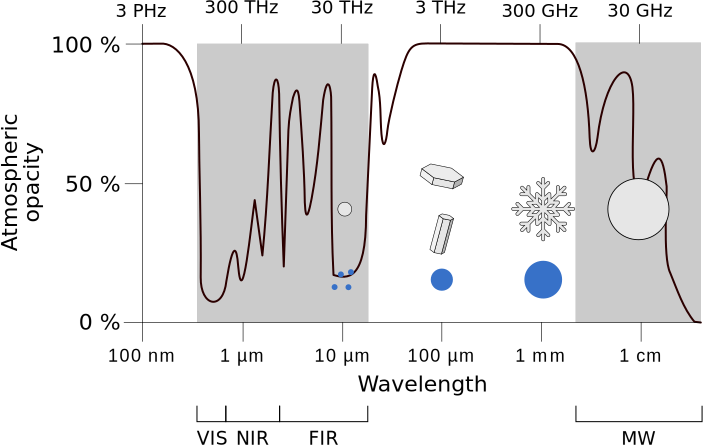
\includegraphics[width=0.75\textwidth]{spectrum}
  \caption{Overview of the electromagnetic spectrum used for hydrometeor retrievals. The black
    curve shows the variation of the atmospheric opacity across the spectrum.}
  \label{fig:radiative_transfer:spectrum}
\end{figure}
%
The discussion presented here focuses on observations from the visible (VIS,
$\SI{350}{\nano \meter} \leq \lambda < \SI{720}{\nano \meter}$), infrared (IR,
$\SI{0.72}{\micor \meter} \leq \lambda < \SI{20}{\micro \meter}$), and microwave
(MW, \SI{1}{\milli \meter} \leq \lambda < \SI{1}{\meter}$) regions, which are
most commonly used for the remote sensing of clouds and precipitation.

An overview of the electromagnetic spectrum is provided in
Fig.~\ref{fig:radiative_transfer:spectrum}. The graph provides an approximate
description of the atmospheric opacity across different wavelengths of the
electromagnetic spectrum. When viewed from a satellite, the atmospheric
opacity defines how far down into the atmosphere a sensor can 'see'. Generally,
where the opacity is low, the satellite can see down to the surface, while where
it is high it is sensitive only to the upper parts of the atmosphere.

\subsection{The atmospheric background}

Satellite observations are sensitive not only to clouds but also to the
gases and aerosols in the atmosphere. As a first approximation the
observations in the absence of clouds, so called \texit{clearsky} scenes,
may be viewed as the background upon which clouds are observed.

Observations at short wavelengths differ from those at long wavelengths with
respect the source of the observed radiation. At wavelengths in the visible and
near infrared regions, the largest part of the observed radiation stems from the
sun. This is because, at these short wavelengths, black body radiation at
typical atmospheric temperatures is small compared to reflection of solar
radiation. As the wavelength increases, the intensity of solar radiation decreases
while that of a black bodies at atmospheric temperatures increases. At wavelengths
exceeding $\approx \SI{3}{\micro \meter}$ emission from atmospheric constituents
dominates the intensity of reflected solar radiation. This threshold separates
the thermal ($\lambda \geq \SI{3}{\mico \meter}$) from the near infrared. At
these wavelengths solar emission can generally be neglected and all observed
radiation originates from the atmosphere itself or the Earth's surface.

The atmospheric opacity displayed in Fig.~\ref{fig:radiative_transfer:spectrum}
corresponds to the combined effects of absorption and extinction by gases in the
atmosphere. Gases affect radiation mostly through absorption and emission, while
scattering plays a role only in the visible range. The reason for this is the
small size of the molecules (around $\SI{1}{\nano \meter}$) compared to the
wavelengths of the radiation.

There is little absorption in the visible range with most of it due to water
vapor. In the near and thermal infrared absorption increases but is concentrated
in discrete absorption bands, which makes the opacity of atmosphere highly
variable across wavelengths. The principal gaseous absorbers in the infrared
region are water vapor, cabon dioxide and ozone. Absorption also plays an
important role in the microwave region with significant contributions from water
vapor, oxygen and ozone. 

In addition to the effects of gases, satellite observations can be affected by
the presence of aerosols. Aerosols are significantly larger than the gas
molecules in the atmosphere and therefore affect both VIS and IR observations
through scattering. In the shortwave part of the electromagnetic spectrum, which
is dominated by solar radiation, aerosols reflect incoming solar radiation and
which typically increases the intensity of the measured radiation due to the
relative darkness of the surface. In the longwave infrared region, the
scattering of aerosols acts to decrease the intensity of the upwelling radiation
from the surface and the lower parts of the atmosphere. Aerosols have no
significant effect on microwave observations.

\subsection{Physical properties of hydrometeors}

Also displayed in Fig.~\ref{fig:radiative_transfer:spectrum} are the principal
classes of hydrometeors located at the wavelengths corresponding to their
approximate sizes. Liquid hydrometeors are identified using blue coloring, while
white corresponds to frozen hydrometeors.

Among the smallest hydrometeors are liquid cloud droplets with typical sizes
around $\SI{10}{\micro \meter}$. These droplets make up liquid clouds. At sizes
of around $\SI{100}{\micro \meter}$ water drops become large enough to fall out
of the clouds. The smallest precipitating liquid droplets are drizzle. These
drops have characteristic sizes of around $\SI{100}{\micro \meter}$. Rain drops
are larger with typical drop sizes around $\SI{1}{\milli \meter}$.

Very small frozen hydrometeors typically form though homogeneous freezing at
temperatures below $-\SI{36}{\degree \celsius}$. Since they require very low
temperatures to form, these hydrometeors are only found at high altitudes.
Larger ice crystals typically form at higher temperatures and lower altitudes.
These range in size from $\SI{100}{\micro \meter}$ to $\SI{1}{\milli \meter}$.
Snow flakes are aggregates of ice crystals that form through collision. These
rang in size from several millimeters to centimeters. When snowflakes fall through
layers that are supersaturated with respect to liquid water, the water vapor
condenses upon the snowflakes causing further growth through a process called
riming. Rimed snowflakes are referred to as graupel and have typical sizes
of $\SI{1}{\centi \meter}$.  Finally, the largest hydrometeors are hailstones,
which form only in strong thunderstorms and can reach sizes of up to
$\SI{10}{\centi \meter}$$.


%Most observations of clouds are affected not only by the clouds themselves but
%also by other constituents of the atmosphere. In the following, we will
%therefore first discuss observations without clouds, so called \textit{clear
%  sky} observations, as these form the background for the observations of
%hydrometeors. This is followed by a discussion of the observable effects of
%hydrometeors on the observations, which gives rise to the signal in the
%\textit{all-sky observations} that can be used to infer the physical properties
%of hydrometeors.

%\subsection{The Earth's surface}
%
%The characteristics of the Earth's surface vary considerably across the
%electromagnetic spectrum. In the visible range, the surface absorbs large parts
%of the radation. The darkest surfaces are the ocean which absorbs around
%$\SI{95}{\percent}$ of the incoming radiation. Bare land surface and forests are
%considerable brighter but still absorb most ($\approx \SI{75}{\percent}$) of the
%incoming radiation. In contrast to that, snow and ice covered surface reflect
%nearly all of the incoming radiation and thus appear very bright.
%
%In the infrared region of the electromagnetic spectrum the emissivity of the Earth surface
%increases significantly. For wavelengths between $3$ and $\SI{20}{\micro \meter}$ the emissivity
%of most surface types is larger than $0.9$. At these wavelengths the surface is very effective at
%emitting and absorbing radiation and there is little contrast between different surface types.
%
%In the microwave region surface emissivity patterns are more complex. Emissivity
%from land is relatively high, while emissivity from water surfaces is low. The
%contrast between land and surface increases with the wavelength. Emissivities
%from snow and ice are lower than that of most bare land surface but higher than
%that of water. The emissivity furthermore depends on the viewing angle and the
%polarization of the radiation.
%
%While these general tendencies are helpful for a qualitative analysis of
%satellite imagery, it should be noted that they only provide a rough
%characterization of the behavior of the Earth's surface across the
%electromagnetic spectrum. Accurate, quantitative modeling of surface
%emissivities is still an unsolved problem and thus remains an area of
%active research.

\subsection{Cloudy sky}

Due to their comparably large sizes, the scattering effects of hydrometeors need
to be taken into account across most wavelengths from the VIS to the MW regions.
In the VIS and NIR there is little absorption from either water or ice.
Hydrometeors thus mostly deviate radiation from its propagation path without
significantly decreasing its intensity. Clouds observed at these wavelengths
appear bright because the solar radiation scattered back towards the sensor is
much more intense than what is reflected from the surface.

In the FIR region, both water and ice are strongly absorbing. Because the
ambient temperature decreases with altitude in the troposphere, opaque clouds
emit less intense radiation than the surface or water vapor below them.
At wavelength at which there is weak absorption from water vapor, so called
\textit{window channels}, radiation from opaque clouds can be used to
infer the temperature at the cloud top, which is related to the altitude of
the cloud.

At microwave frequencies, liquid water is a much more efficient absorber than
ice. Because of this, absorption and emission from ice can be neglected. At
frequencies below $\sim \SI{50}{\giga \hertz}$, the scattering from hydrometeors
becomes negligible. Because of that the dominant impact of hydrometeors on
satellite observations is through the emission from liquid hydrometeors. Over
Ocean surfaces, which have low emissivity and thus emit little radiation, the
emission from liquid hydrometeors causes a clear signal in microwave
observations at these low frequencies.

At frequencies above $\SI{50}{\giga \hertz}$, observations become
sensitive to the scattering from snow flakes. This scattering signal is
important for sensing precipitation over land, where the emission signature from
liquid hydrometeors may not be detectable due to the much warmer background
surface.

\section{Satellite remote sensing}

Just as the interaction of hydrometeors with electromagnetic radiation,
also the information content of the satellite observations  on specific
hydrometeors varies with the wavelength. However, the observation frequency
can in general not be chosen freely but is subject to technological
limitations, which affect characteristics such as spatial and temporal
resolution of the observations.


\subsection{Satellite orbits}

The satellite orbit in which the satellite and sensor are placed plays an
important role in determining the characteristics of the resulting observations.
Geostationary satellites orbit the Earth at the same angular velocity as the
Earth itself.  This allows
them to hover over the same position of the Earth surface. Since the field of
view of the satellite is constant it can provide observations with high temporal
resolution at all locations below the satellite. This makes these satellite
suitable for many near real-time applications in weather forecasting.

The disadvantage of geostationary platforms is their long distance from the
Earth, which is around $\SI{35\ 000}{\kilo \meter}$. This makes them unsuitable
for microwave sensors, whose resolution is diffraction limited and would thus
require a very large antenna to achieve low spatial resolution. Geostationary
satellites therefore typically carry VIS and IR sensors, which can produce
observations with very high spatial resolution.

Earth observing satellites commonly placed into polar or sun-synchronous orbits,
which are much lower than geostationary orbits. The low altitude of these orbits
($300 - \SI{1000}{\kilo \meter}$) makes them suitable for microwave sensors.
Although the low altitude favors high spatial resolution, it decreases the
spatial coverage of the sensor. The swaths of sensors in these low-earth orbits
are typically limited to a few thousand kilometers in width. Depending on the
exact size of the field of view and the location on Earth, the time between
consecutive overpasses for a fixed position be as high as $\SI{12}{\hour}.

Fig.~\ref{fig:remote_sensing:viewing_geometries} shows the field of views of
the Advanced Baseline Imager on the GOES 16 geostationary satellite and the
GPM Microwave Imager on the polar-orbiting GPM Core Observatory. The observations
from both satellites are projected onto the corresponding location on the Earth.
This illustration clearly shows the differences that the satellite orbit makes
for the observations. While the geostationary satellite can permanently observe
a large part of the hemisphere below it, the polar orbiting satellite sees only
a comparably thin stripe of the globe.

\begin{figure}[!hbpt]
  \centering
  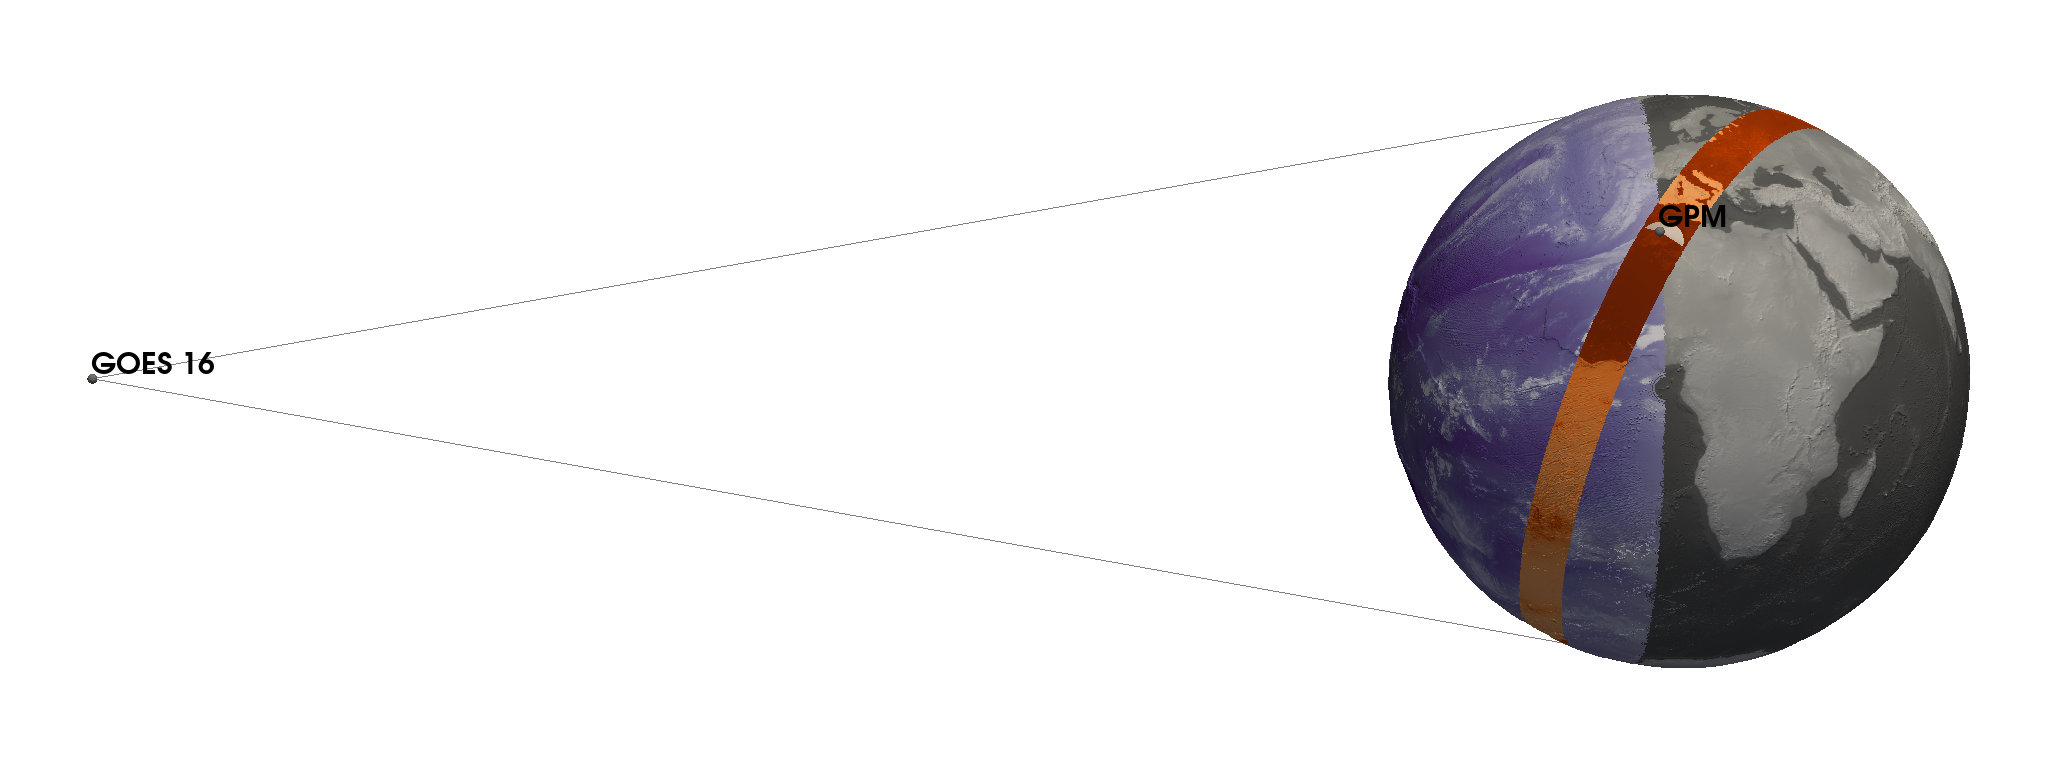
\includegraphics[width=0.8\textwidth]{viewing_geometries}
  \caption{Viewing geometries of geostationary and polar-orbiting satellites
  drawn to scale. The illustration shows geo-located satellite observations from
  the GOES 16 geostationary satellite in purple and from the polar-orbiting GPM
  Core Observatory in orange. The black spheres mark the instantaneous satellite
  positions.}
  \label{fig:remote_sensing:viewing_geometries}
\end{figure}




\subsection{Sensor types}

In addition to \texit{passive} sensors, which sense reflected solar radiation or
thermal radiation emitted from the Earth or its atmosphere, there exist sensors
that themselves emit radiation and measure the amount of it that is scattered
back to the sensor. By measuring the time of travel between emission and
reflection, these \textit{active} sensors measure the distance from the detector
in addition to the intensity of the reflected radiation this allows them to
profile the atmosphere along the line of sight, which leads to much higher
vertical resolutions than what can be achieved with atmospheric sounding.

\subsection{Example: Satllite observations of Hurricane Ida}

Figure~\ref{fig:radiative_transfer:observations} illustrates the different types
of observations used for the remote sensing of hydrometeors using observations
of Hurricane Ida. The first row of panels shows observations derived from the
Advanced Baseline Imager on the GOES 16 geostationary satellite. Panel (a) shows
a natural color composite, which combined observations from 3 channels from the
VIS and NIR to create an image that human color vision. Panel (b) shows
observations from the NIR. Differences in the dielectric constant of water and
ice cause ice clouds to absorb incoming solar radiation much more strongly than
water clouds. The high ice clouds that cover the Hurricane therefore appear much
darker than in the RGB image. Panel (c) shows observation from a window channel
in the FIR. Since it is a window channel, most of the radiation observed in
cloud free areas stems from the Earth's surface and thus appear bright. Where
clouds are present the observed brightness temperatures are closely related to
the atmospheric temperature at the altitude of the cloud and thus colder than
the surface.

Panel (c) and (d) show passive microwave observations at $\SI{18.7}{\giga
  \hertz}$ and $\SI{166}{\giga \hertz}$. At the very low microwave frequencies
only the a thermal emission from precipitation in the hurricane is visible over
the cold ocean surface, while the clouds overland yield no signal. At the higher
microwave frequencies, the surface is not visible due to emission from water
vapor. Scattering by snow particles causes a cold scattering signal from the
thickest clouds around the Hurricane.

Finally, panel (e) shows Ku-band radar reflectivities from the GPM
dual-frequency precipitation radar along a vertical cross section of the
Hurricane. The signal in the radar observations is the amount of energy that is
reflected back to the sensor. Due to the relatively low frequency of the
radar, it is only sensitive to large, precipitation hydrometeors.


\begin{figure}
  \centering
\includegraphics[width=\textwidth]{observations}
\caption{Satellite observations of Hurricane Ida on 2021-08-29 15:09 UTC.
  Panels (a), (b), (c) show observations from the VIS and IR regions obtained
  by the Advanced Baseline Imager on the GOES 16 geostarionary satellite.
  Panels (d) and (e) show passive microwave observations from the GPM microwave
  imager. Panel (f) shows the curtain of radar reflectivity measured by the GPM dual-frequency
  precipitation radar (DPR) along the dashed line shown in panel (a).}
\label{fig:radiative_transfer:observations}
\end{figure}


\chapter{Satellite remote sensing of clouds and precipitation}

The interactions of hydrometeors with electromagnetic radiation, which were
discussed in the previous chapter, provide the signal that can be measured
by earth observing satellites. This chapter now turns to the practical
aspects of the remote sensing of hydrometeors, namely how these signals
can be obtained and how they can be related into physical estimates.

\section{Satellite observations}



\subsection{Synergies}

\section{Satellite platforms}

\section{Satellite observations}


\section{Observation frequencies}

At visible and infrared wavelengths the scattering and absorption by clouds are
so strong that these observations are sensitive only to cloud tops. While this
helps to determine the altitude of the clouds as well as the properties of the
particles in those upper parts, these observations contain only indirect
information on the lower parts of the cloud or the occurrence of precipitation.

In the microwave domain, the interaction between radiation and hydrometeors are
much weaker. At frequencies below around $\SI{50}{\giga \hertz}$ the only signal
observed is emission from rain drops. This, however, requires a relatively dark
background and therefore typically only visible above water surfaces. At
frequencies between about $50$ and $\SI{200}{\giga \hertz}$ scattering from large
snow flakes causes a cold scattering signal in the warmer upwelling radiation.
Observations at these long wavelengths can thus provide information only on the
largest particles in the cloud, which are typically so large that they are
precipitating in the form of rain, snow, graupel or hail.




\chapter{Machine learning}
Radiative transfer theory describes how radiation that interacts with
hydrometeors produces an electromagnetic signal in satellite observations. Since
the purpose of the observations is to provide information on the physical
properties of hydrometeors, a way must be found to relate the observations to
those properties. This process is referred to as retrieval. This chapter
presents the mathematical formulation of the retrieval problem and provides a
brief introduction to the machine-learning-based methods to solve it.

\section{The retrieval problem}
\label{sec:machine_learning:retrieval_problem}

% So how can these observations be turned
%into estimates of physical properties? This is not a simple task because the
%observations are typically affected by non-negligible measurement noise and,
%more importantly, are generally ambiguous in the sense that physically different
%atmospheric states can produce nearly identical observations.

Mathematically, the problem of determining properties of hydrometeors from
satellite observations can be formulated as finding a state vector%
\footnote{ The notation for the state and observation vectors was deliberately
chosen to be the opposite of the conventions of inverse problem theory to make
it consistent with the conventions used in machine learning. }
$\vec{y} \in \mathrm{R}^{n}$ that describes the physical properties of the atmosphere from a
vector of observations $\vec{x} \in \mathrm{R}^{m}$. This so-called
\textit{retrieval problem} can be solved using the mathematical framework of
inverse problem theory. In inverse problem theory, the underlying assumption is
that the observations $\vec{x}$ are generated by a physical processes, which
can be described using a forward model function $f: \mathrm{R}^n \rightarrow
\mathrm{R}^m$, but may be affected by a random error $\vec{\epsilon} \in
\mathrm{R}^M$:
\begin{align}\label{eq:inverse_problem}
  \vec{x} &= f(\vec{y}) + \vec{\epsilon}
\end{align}

An exact solution to this problem does not exist. Because of the random noise
$\vec{\epsilon}$, the equation can never be strictly satisfied. Furthermore,
there usually exist many states $\vec{y}$ that produce similar measurements
$\vec{x}$, thus rendering the problem underconstrained. Since it does not
admit a unique solution, the retrieval problem is \textit{ill-posed}.

Although an exact solution to the retrieval problem is not possible, Bayesian
statistics provides a framework to extract the available information from the
observations. In the Bayesian approach, both the observations $\vec{x}$ and the
atmospheric state vector $\vec{y}$ are assumed to be random variables.
Furthermore,  it is assumed that $\vec{y}$ is distributed according to a known
\textit{a priori} distribution $p(\vec{y})$. Instead of a single, unique state
$\vec{y}$, the solution of the problem then becomes the \textit{a posteriori} (or
\textit{posterior}) distribution $p(\vec{y} | \vec{x})$ of the atmospheric
state. According to Bayes theorem, the a posteriori distribution for given
observations $\vec{x}$ is given by
\begin{align}\label{eq:bayes}
  p(\vec{y} | \vec{x}) &= \frac{p(\vec{x}|\vec{y})
  p(\vec{y})}{p(\vec{x})}.
\end{align}
Traditionally, Bayesian methods for solving the retrieval problem make use of
the right-hand side of Eq.~\ref{eq:bayes} to approximate the posterior
distribution. The approach pursued in this thesis is to learn the posterior
distributions $p(\vec{y}|\vec{x})$ directly from data. How this can be done is
the topic of the remainder of this chapter.

\section{Machine learning}


The field of machine learning is concerned with the development of algorithms
that can learn to solve computational tasks from data. More specifically, the
methods considered here solve the problem of \textit{supervised learning}. In
supervised learning, the task is to learn how to produce a certain output
$\vec{y}$ from inputs $\vec{x}$ given a set of pairs $\{(x_i, y_i)\}\text{ for
}i = 1, \ldots, N$ of specific input values $\vec{x}_i$ and corresponding output
values $\vec{y}_i$. In general, the inputs $\vec{x}$ and outputs $\vec{y}$ may
represent anything from simple numbers to images or texts. For the applications
considered here, the inputs are typically satellite images, and the outputs are
the corresponding physical quantities to be retrieved.

Machine learning has gone through a wave of immense popularity during the 2010s
triggered by the success of \textit{deep learning} methods in addressing a range
of computational problems in computer vision, natural language processing, and
artificial intelligence. The idea behind deep learning is to construct
increasingly powerful models from a hierarchy of simple models. Given sufficient
data, these models can learn highly complex relationships and require less
guidance from human experts to achieve good performance.

\subsection{Shallow machine learning}

Although the focus of this thesis is deep learning, this section will use a very
shallow model to illustrate the basic principles of machine-learning-based
remote sensing retrievals. The considered example tries to estimate rain at the
surface from infrared (IR) observations at a wavelength of $\lambda =
\SI{10.3}{\micro \meter}$. The training data, which contains of the in- and
outputs from which a solution to the retrieval problem should be learned, is
derived from co-locations of observations from the GOES 16 geostationary
satellite and the combined radar and passive microwave retrievals from the GPM
core observatory (see Sec. \ref{sec:radiative_transfer:synergies}).

The input $x$ for this particular example corresponds to the measured radiation
at a single pixel of the geostationary observations while the output $y$ is
given by the rain rate measured by the GPM core observatory. The retrieval
assumes a linear relationship between the observations $x$ and the rain rate $y$
in order to determine the precipitation corresponding to the geostationary
observations:
\begin{align}
  y &= a x + b
\end{align}
The two parameters of the linear regression model are the slope $a$ and 
the intercept $b$. They can be determined by finding the values that minimize the
squared error between the predictions and the true rain rates.

Panel (a) in Fig.~\ref{fig:machine_learning:linear_regression} shows the
distribution of the training data together with the learned relationship between
input and output data. This view reveals that the relationship is not very
robust, which becomes even clearer when the retrieval results (panel (b)) are
compared to the reference precipitation (panel (c)). The linear regression model
simply predicts rain almost everywhere where there is a cloud but completely
fails to reproduce the structure in the reference precipitation.

\begin{figure}
  \centering
  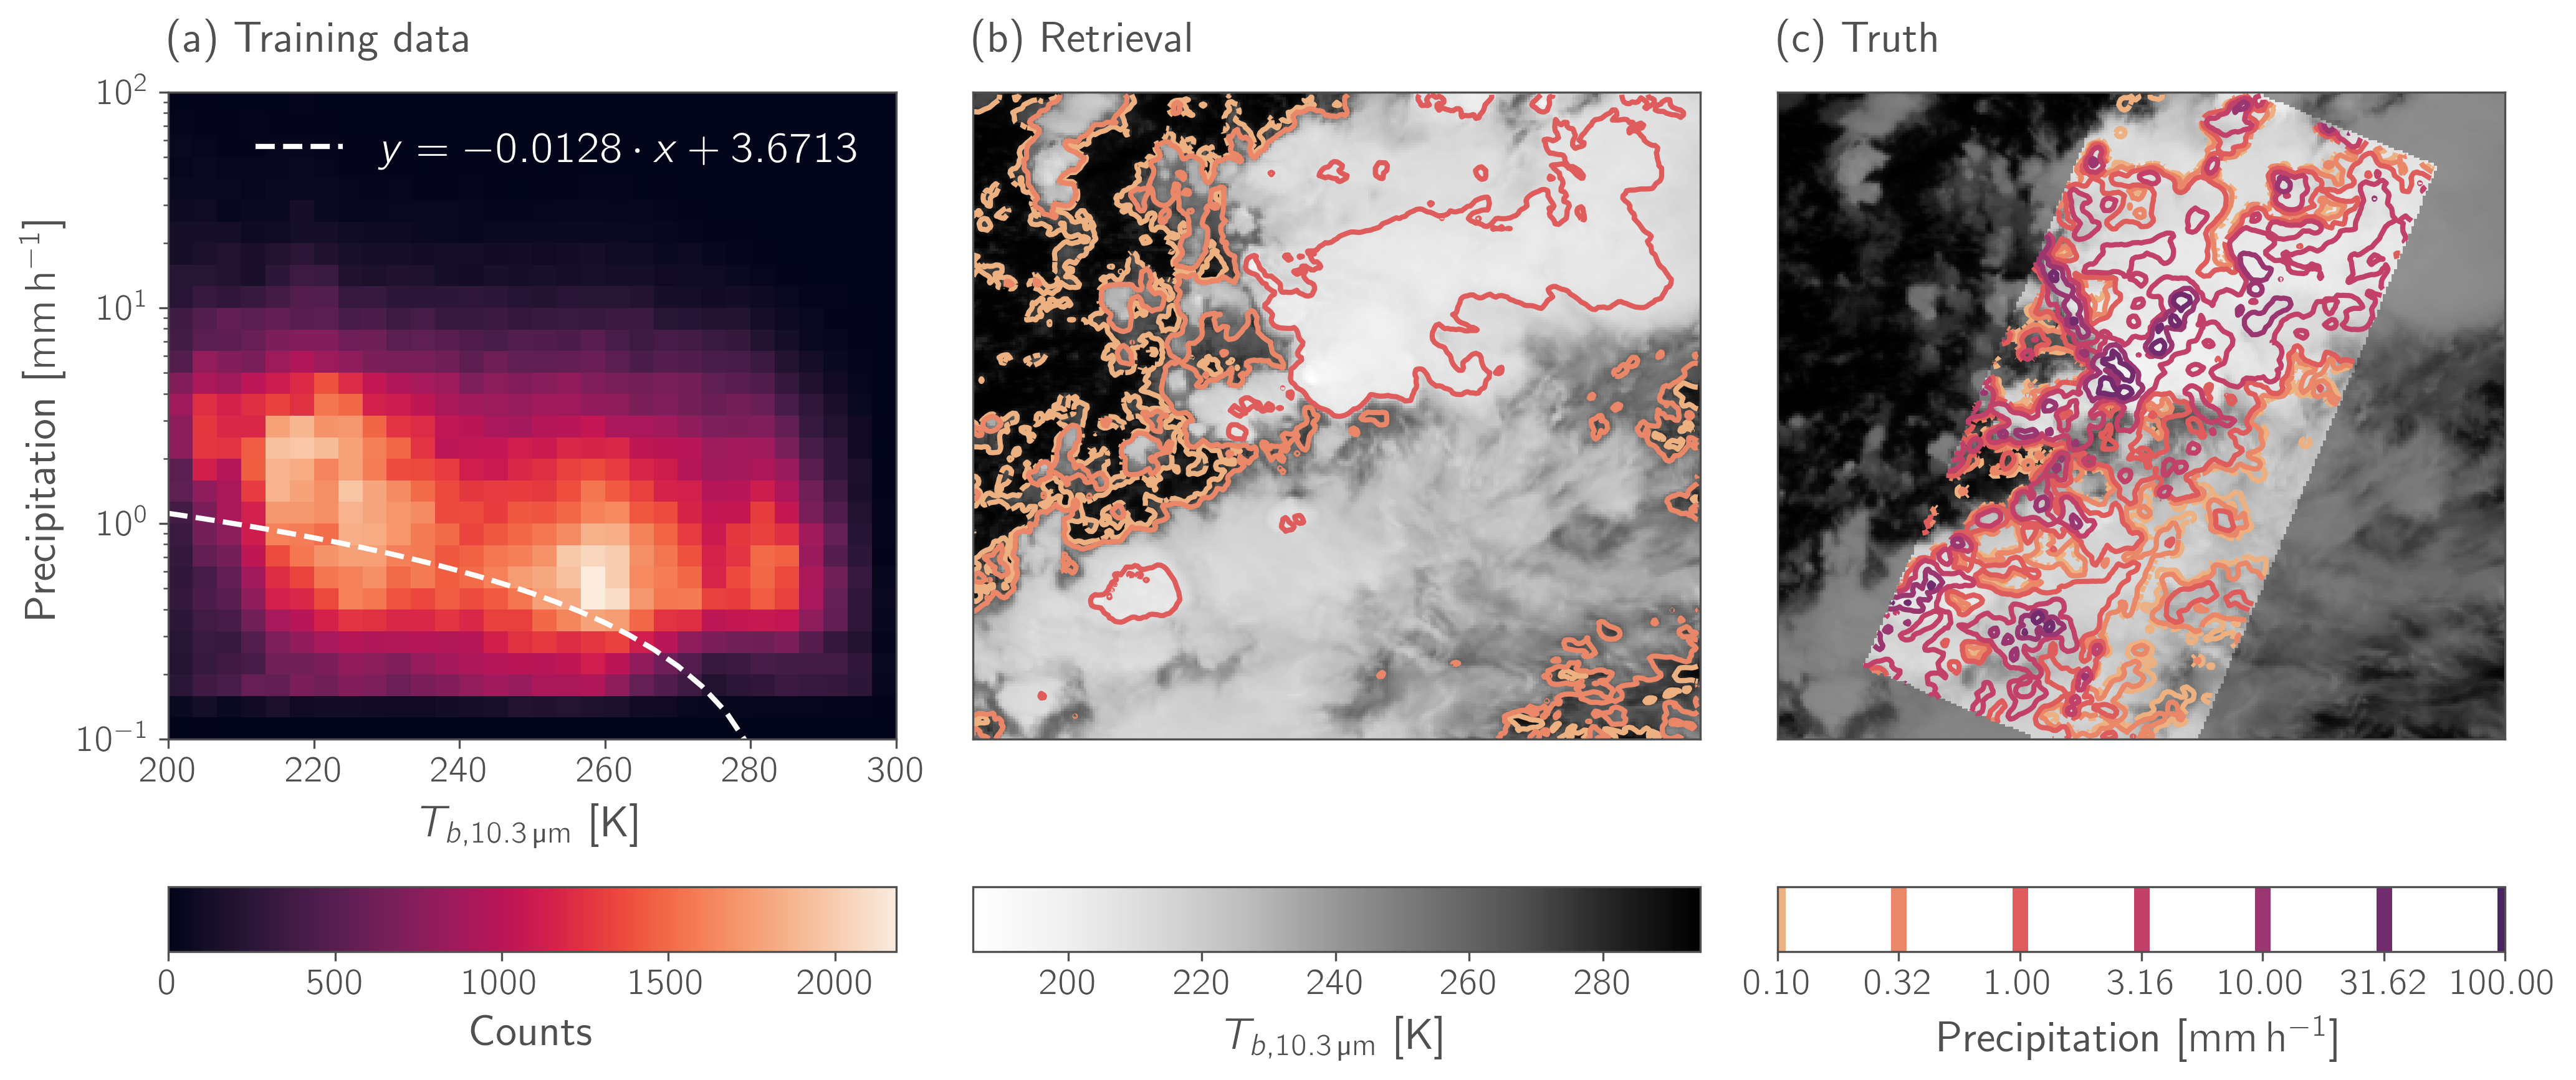
\includegraphics[width=\textwidth]{linear_regression.png}
  \caption{Example of a very simple precipitation retrieval. Panel (a) shows a
    density plot of the distribution of the input-output pairs, which consist of
    IR brightness temperatures and surface precipitation rates. The white line
    shows the linear relationship between observations and rain rate obtained by
    linear regression. Panel (b) shows retrieved precipitation rates when the
    learned relationship is applied to real observations. Panel (c) shows the
    true precipitation rates as present in the training data. Because of the
    narrow swath of the GPM precipitation radar the precipitation is not known
    across the full scene. }
  \label{fig:machine_learning:linear_regression}
\end{figure}

Given the bad performance of the simple linear regression model, it is natural
to ask how a better-performing model can be found. In general, there are three
dimensions along which a machine learning model can be improved:
\begin{description}
\item[Model expressivity:] The model used in this example can only learn
  linear relationships between input and output. The range of mathematical functions
  that a model can represent is referred to as its \textit{expressivity}. Increasing
  the model expressivity enables it to learn  more complex relationships between
  the input and output.
\item[Amount of input information:] The scatter plot in panel (a) of
  Fig.~\ref{fig:machine_learning:linear_regression} shows that the problem of
  retrieving precipitation from infrared (IR) observations is highly degenerate. For any
  value of the observations, the training data contains a wide range of different precipitation
  values. This makes it impossible to assign a unique `right' precipitation rate
  to an observed brightness temperature. The degeneracy can be decreased by
  adding more information to the input. One way to achieve this, for example, is
  to add observations from other channels or information from neighboring
  pixels. Depending on the problem, this may provide  more flexibility
  to distinguish different precipitation rates to the model.
\item[Amount of data:] A machine learning model can only learn relationships
  that are sufficiently well represented in the training data. For more complex
  retrievals than this one, larger amounts of training data are crucial for good
  retrieval performance.
\end{description}

Traditionally, the difficulty in improving a machine learning model was that it
is not sufficient to just increase the model expressivity or the amount of input
information. Both measures increase the flexibility of the model and may
thus cause it to \textit{overfit}. Overfitting occurs when the
model learns spurious relations from the training data, which are not actually
representative of the true relationship between input and output. This typically
causes predictions on unseen data to deteriorate drastically. Overfitting can be
counteracted by artificially reducing the expressivity of the model, a process
that is called \textit{regularization}, as well as by increasing the amount of data
that is used to train the model. However, the time and computational resources
that are required for training typically increase with the amount of data. If
the  increase is too rapid, the amount of data that a machine learning model
can be trained on may be limited.

Because of this, machine learning models traditionally depend on careful tuning
to the task at hand. Especially the trade-off between model expressivity and the
amount of data that can be used to train it required a multi-disciplinary
approach that combined domain-specific knowledge with machine-learning
experience to develop a good-performing model. A particular difficulty of
shallow models was their inability to handle large inputs with low information
density, such as the pixels from an image. Providing a shallow model with too
many inputs typically makes the models prone to overfitting and more difficult
to train. This gave rise to the practice of \textit{feature engineering}, which
consists of manually designing input variables that encode high-level
information in task-specific input features.

It should be noted that the linear regression model used here is extremely
simple and that there exist shallow machine learning methods that would likely
work much better for this example. Nonetheless, the application is not totally
unrealistic, given that it is similar to early precipitation retrievals from
geostationary observations \citep{vicente98}. To overcome the limitations of the
linear regression, the model from \citet{vicente98} predicts precipitation in
log-space and uses weather model data to post-process the retrieval results.
Modified versions of this retrieval are still in operational use today
\citep{siqueira19}.

\subsection{Deep learning}

The example discussed above illustrated the limitations of very shallow machine
learning methods that deep learning aims to overcome. The essential promise of
deep learning is that it decouples the dimensions along which a machine learning
model can be improved. Deep learning models achieve high expressivity by
stacking a large number of simple models and maximizing the amount of input
data. Since the training time of deep learning methods scales linearly with the
amount of available data while the required memory remains constant, the
increased model expressivity can be balanced with large amounts of training
data. This enables deep learning models to learn highly complex relationships
from data without the risk of overfitting.

  \subsection{Neural networks}

  Seen from a more general perspective, the linear regression model considered
  above is just a transformation from the input $x$ into the output $y$ with a
  set of learnable parameters, in this case, the slope and intercept of the
  regression. A neural network is just a sequence of such parametrized
  transformations, which are referred to as \textit{layers}. Each layer
  transforms an input vector into an output vector, which is passed on to the
  next layer. The exact form of each transformation can be adapted through its
  parameters, which is done by minimizing an error metric over the training
  data.

  Defined in this way, every neural network also satisfies the definition of a
  layer. This allows any neural network to be used as a component within a
  larger network.

  %sAn important characteristic of this definition of a neural network is its
  %recurrence: A neural network is itself a transformation of an input vector
  %into an output vector and may thus be used as a layer in a larger network. At
  %the same time, however, this makes the definition of what exactly constitutes a
  %layer in a network somewhat arbitrary.

  \subsubsection{The multi-layer perceptron}

  Extending the simple linear regression model to accommodate for multiple in-
  and outputs yields one of the most fundamental transformations used in neural
  networks. It is typically referred to as \textit{linear} or \textit{fully-} or
  \textit{densely-connected} layer. Mathematically, this layer implements an
  affine transformation of the input vector $\bm{x}$ of the form
  \begin{align}
    \bm{y} = \bm{W}x + \bm{b}
  \end{align}
  where $\bm{W} \in \mathrm{R}^{m \times n}$ is a matrix of weights $W_{i,j}$,
  and $\bm{b} \in \mathrm{R}^m$ a vector of  biases.

  Fully-connected layers are typically used in combination with a non-linear
  function that is applied element-wise to its inputs. These functions are
  called \textit{activation functions}. Without them, stacking fully-connected
  layers does not increase the expressivity of the neural network, which in this
  case depends only on the number of input and output variables.

  There exist a wide range of activation functions. One of the currently most
  commonly used activation functions in deep neural networks is the Rectified
  Linear Unit (ReLU).
  \begin{align}
    \text{ReLU(x)} = \begin{cases}
      x & x > 0 \\
      0 & x \leq 0
    \end{cases}
  \end{align}
  It should be noted, however, that neural network architectures are an area of
  active research and several alternatives and modifications of the ReLU
  activation have been proposed.

  A neural network consisting of one or several layers of fully-connected
  layers followed by activation functions is typically referred to as
  multi-layer perceptron (MLP). Since all numeric inputs can be brought into
  vector form and thus fed into an MLP, the MLP is one of the most fundamental
  forms of neural networks.

\subsubsection{Convolutional neural networks}

Although MLPs can be applied to image data directly by flattening the input into
a single vector, this approach was found to not work well in practice. The
principal reason for this is that the number of parameters in the model becomes
very large, making it prone to overfitting and the training more
difficult.

An important technique in the application of neural networks to image data was
the introduction of the convolutional layer, which replaces the
matrix multiplication of the fully-connected layer by a convolution with a
learnable filter kernel. Let $\bm{X} = [X_{i, j}]$ for $i = 1, \dots, M, j = 1,
\ldots, N$ be an input image of size $M \times N$ and $\bm{K} = [K_{i, j}]$ for
$i = - k \ldots k, j = -k, \ldots, k$ a given convolution kernel of 
size $(2k + 1) \tims (2k + 1)$. In two dimensions, the convolution
operation $\bm{Y} = \bm{X} * \bm{K}$ of
$\bm{X}$ and $K$ used in machine learning is defined as
\begin{align}\label{eq:machine_learning:convolution}
  Y_{i, j} &= \sum_{l=-k}^{k} \sum_{m=-k}^{k} X_{i + l, j + m} K_{i + l, j + m}
\end{align}
This operation corresponds to a filter mask whose response is calculated for all
possible locations in the input image by sliding the filter window across the
width and height of the image. Since digital images, as well as satellite
observations, contain information also along a spectral dimension, the images
actually correspond to three-dimensional tensors with an additional channel
dimension in addition to the two spatial dimensions. To account for this, the
kernel and sum in Eq.~\ref{eq:machine_learning:convolution} are extended across
all channels of the input image.

An illustration of the convolution operation for an input image with multiple
channels is shown Fig.~\ref{fig:machine_learning:convoluation}. The input
corresponds to a rank-three tensor with one channel and two spatial dimensions.
The kernel is limited in its extent in the spatial dimensions but extends over
all channels of the input. A two-dimensional output tensor is obtained by
calculating the kernel activation for all possible locations in the input
tensor. A convolutional layer consists of a set of convolution
kernels. The two-dimensional filter responses of each kernel are stacked along
the channel dimension to produce a rank-three tensor as output of the layer.

In a convolution layer, the convolution operation is typically combined with
the application of a bias term to each element in the output tensor. The learnable
parameters of a convolution layer thus correspond to the elements of each of its
kernels as well as the bias terms for each output.

\begin{figure}
  \centering
  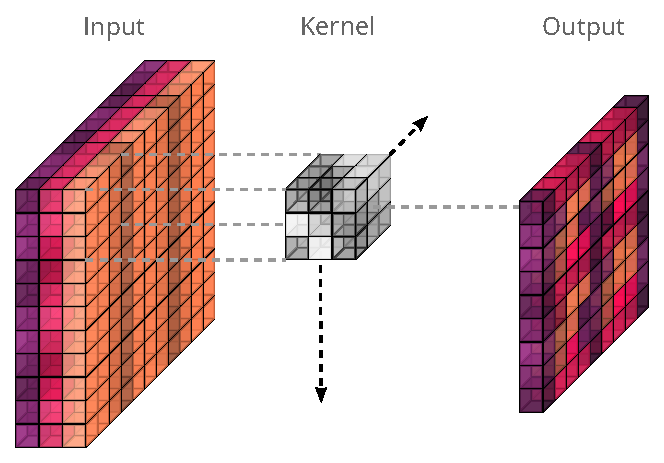
\includegraphics[width=0.5\textwidth]{convolution}
  \caption{
    Illustration of the convolution operation. The output of the convolution
    operation is obtained by applying the filter kernel sequentially to every
    possible position in the input image.
  }
  \label{fig:machine_learning:convoluation}
\end{figure}

Since the convolution transformation is linear, it is a special case of the
fully-connected transformation of the corresponding flattened input image.
However, in the fully-connected case, each pixel in the output image would be
connected by independent parameters to all pixels in the input image, whereas
for the convolutional layers, the parameters are shared between all pixels in a
given channel of the output image. This greatly reduces the number of learnable
parameters of the convolutional layer compared to a fully-connected one.

The convolution encodes two important properties of images into the neural
network model, which are translation invariance and locality. Translation
invariance refers to the property of the convolution operation that its output
is independent of the relative location within the image. It is clear that this
is a suitable assumption for many image processing tasks since features that
identify an object should not be affected by their position in an image. The
property of locality refers to the fact that each output of a convolution layer
is determined only by a limited, connected subset of pixels of the input image,
the number of which depends on the kernel size $k$. This encodes the assumption
that for understanding the content of a given image region only neighboring
pixels should be relevant.

Convolutional neural networks are neural networks built-up of convolution
layers. These networks typically combine convolutional layers with downsampling
layers that successively decrease the size of the input image, which allows these
networks to combine information across the spatial dimensions of the image.

The motivation for this is to allow the model to learn a hierarchy of
transformations from low-level information on the pixel scale to a reduced
amount of high-level information that is relevant to the task that the
network is being trained to solve.

\subsubsection{Training}
%Now that the basic building blocks of modern neural networks have been
%introduced, the question remains how they can be trained to solve a given
%computational task. As mentioned above, we are considering the case of
%supervised learning in which training data in the form of samples from the joint
%distribution of input data $x$ and corresponding outputs $y$ are available.

The basic training approach for neural networks is similar to that of the
fitting of the parameters of a linear regression model, which are found by
minimizing a certain loss criterion over the training data. For linear
regression, this is typically the mean squared error, which can also be used to
train neural networks. In contrast to linear regression, however, the parameter
optimization for the neural network can not be solved explicitly. Instead,
neural networks rely on iterative minimization of the loss function using
gradient descent optimization.

While naive gradient descent would require traversing the whole training dataset
to compute the gradients required to perform a single descent step, it is in
practice sufficient and even beneficial to only use a small subset of samples
from the training data. This modification of traditional gradient descent, which
is known as \textit{stochastic (mini-batch) gradient descent}, allows neural
networks to scale  to very large datasets. In addition to that, the
stochasticity of the calculated gradients prevents the optimization process from
getting stuck in local minima of the cost function.

\subsubsection{Uncertainty in machine learning}

The ill-posed character of the retrieval problem discussed in
Sec. \ref{sec:machine_learning:retrieval_problem} leads to significant
uncertainties in most remote sensing retrievals. In addition to that,
the machine learning approach gives rise to two additional sources
of uncertainties in the retrieval.

%Machine learning techniques allow us to train a model that retrieved physical
%quantities from satellite observations. However, as discussed in
%Sec.~\ref{sec:remote_sensing:retrieval_probem}, there is no unique solution to
%the retrieval problem. Mathematically, this means that any prediction consisting
%of just a single value will always be wrong. Given the impossibility of solving
%the retrieval problem exactly and import questionj becomes whether the model
%learn how wrong it is?

The total error that a machine learning model makes in its prediction is its
\textit{predictive uncertainty}. The predictive uncertainty can be decomposed
into three independent sources. The first one, referred to as \textit{epistemic
  uncertainty}, is the uncertainty caused by a lack of training data. Its
defining property is that it can be reduced by collecting more data to train the
model on. The second type is called \textit{aleatoric uncertainty}. This
uncertainty refers to the uncertainty that cannot be reduced by increasing the
amount of data that the model is trained on. In the context of satellite
observations, this uncertainty is caused by the inability of the observations to
fully determine the observed atmospheric state. It is thus a consequence of the
ill-posed nature of the retrieval problem  discussed in
Sec.~\ref{sec:machine_learning:retrieval_problem}.

An illustration of the concepts of aleatoric and epistemic uncertainty is provided
in Fig.~\ref{fig:machine_learning:uncertainties}. The plot shows the joint
distribution of observations and the retrieval target for a hypothetical retrieval
scenario. The filled contours in the background show the actual joint distribution
that relates the observations to the targets. The grey markers show the
available training samples. If these samples were to be used to train a neural
network model, the uncertainty in the left part of the graph would be dominated
by the aleatoric uncertainty, because the spread of the underlying, true relationship
is well represented in the training data. In the right part of the graph,
however, the training samples are too few to capture the relevant features of
the relationship and uncertainties would be dominated by epistemic uncertainty.

\begin{figure}
  \centering
  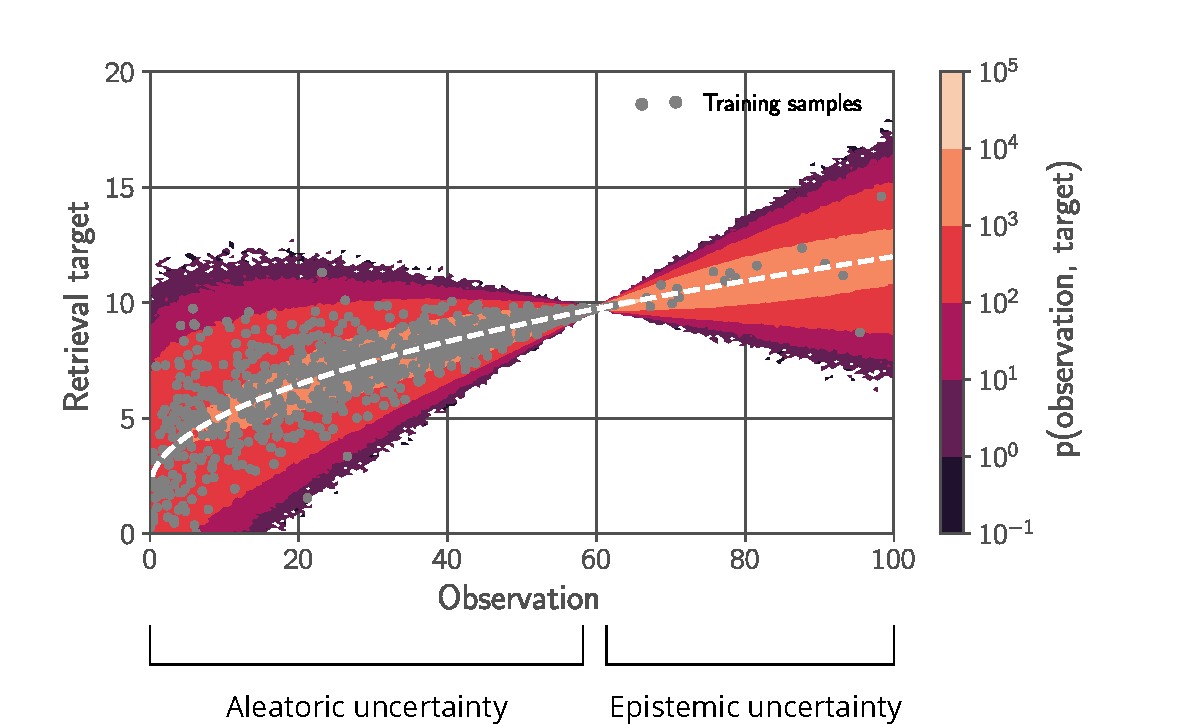
\includegraphics[width=\textwidth]{uncertainties}
  \caption{
    Illustration of aleatoric and epistemic uncertainty. The graph
    displays the relationship between observations and retrieval target
    for a hypothetical retrieval scenario. In the left part of graph the
    uncertainties are dominated by aleatoric uncertainty, whereas in
    the right part they are dominated by epistemic uncertainty.
  }
  \label{fig:machine_learning:uncertainties}
\end{figure}

The final source of uncertainty is caused by differences between the training
data and the data that the model is actually applied on. It is typically
referred to as \textit{covariate shift}. It is obvious that when the wrong data
is used to train the model, it is likely to produce wrong results. However,
subtle changes between training data and the actual data that the model is
applied on are not uncommon and can  increase the predictive uncertainty of
the model.

\subsection{Revisiting the precipitation retrieval}

To provide a demonstration of the capabilities of the deep learning methods,
Fig.~\ref{fig:machine_learning:retrieval_comparison} revisits
the retrieval example introduced above and displays the results from two additional
retrievals, which have been trained using the same data.

The first one is based on an MLP, which uses the same single-pixel input as the
linear regression model. The results from this retrieval are shown in panel (b).
Compared to the reference precipitation shown in panel (d), the results show
modest improvements in the structure of the precipitation, but its spatial
extent is still strongly overestimated. Since the MLP uses only information from
a single input channel, it is severely limited in the relations that it can
learn. It is therefore not surprising that it does not work much better than the
linear regression model.

To explore the full potential of deep learning methods, the second model uses a
CNN to retrieve precipitation using the full input image and all 16 channels of
the geostationary observations simultaneously. These results show clear
improvements both in the structure of the retrieved precipitation as well as its
spatial extent.

\begin{figure}
  \centering
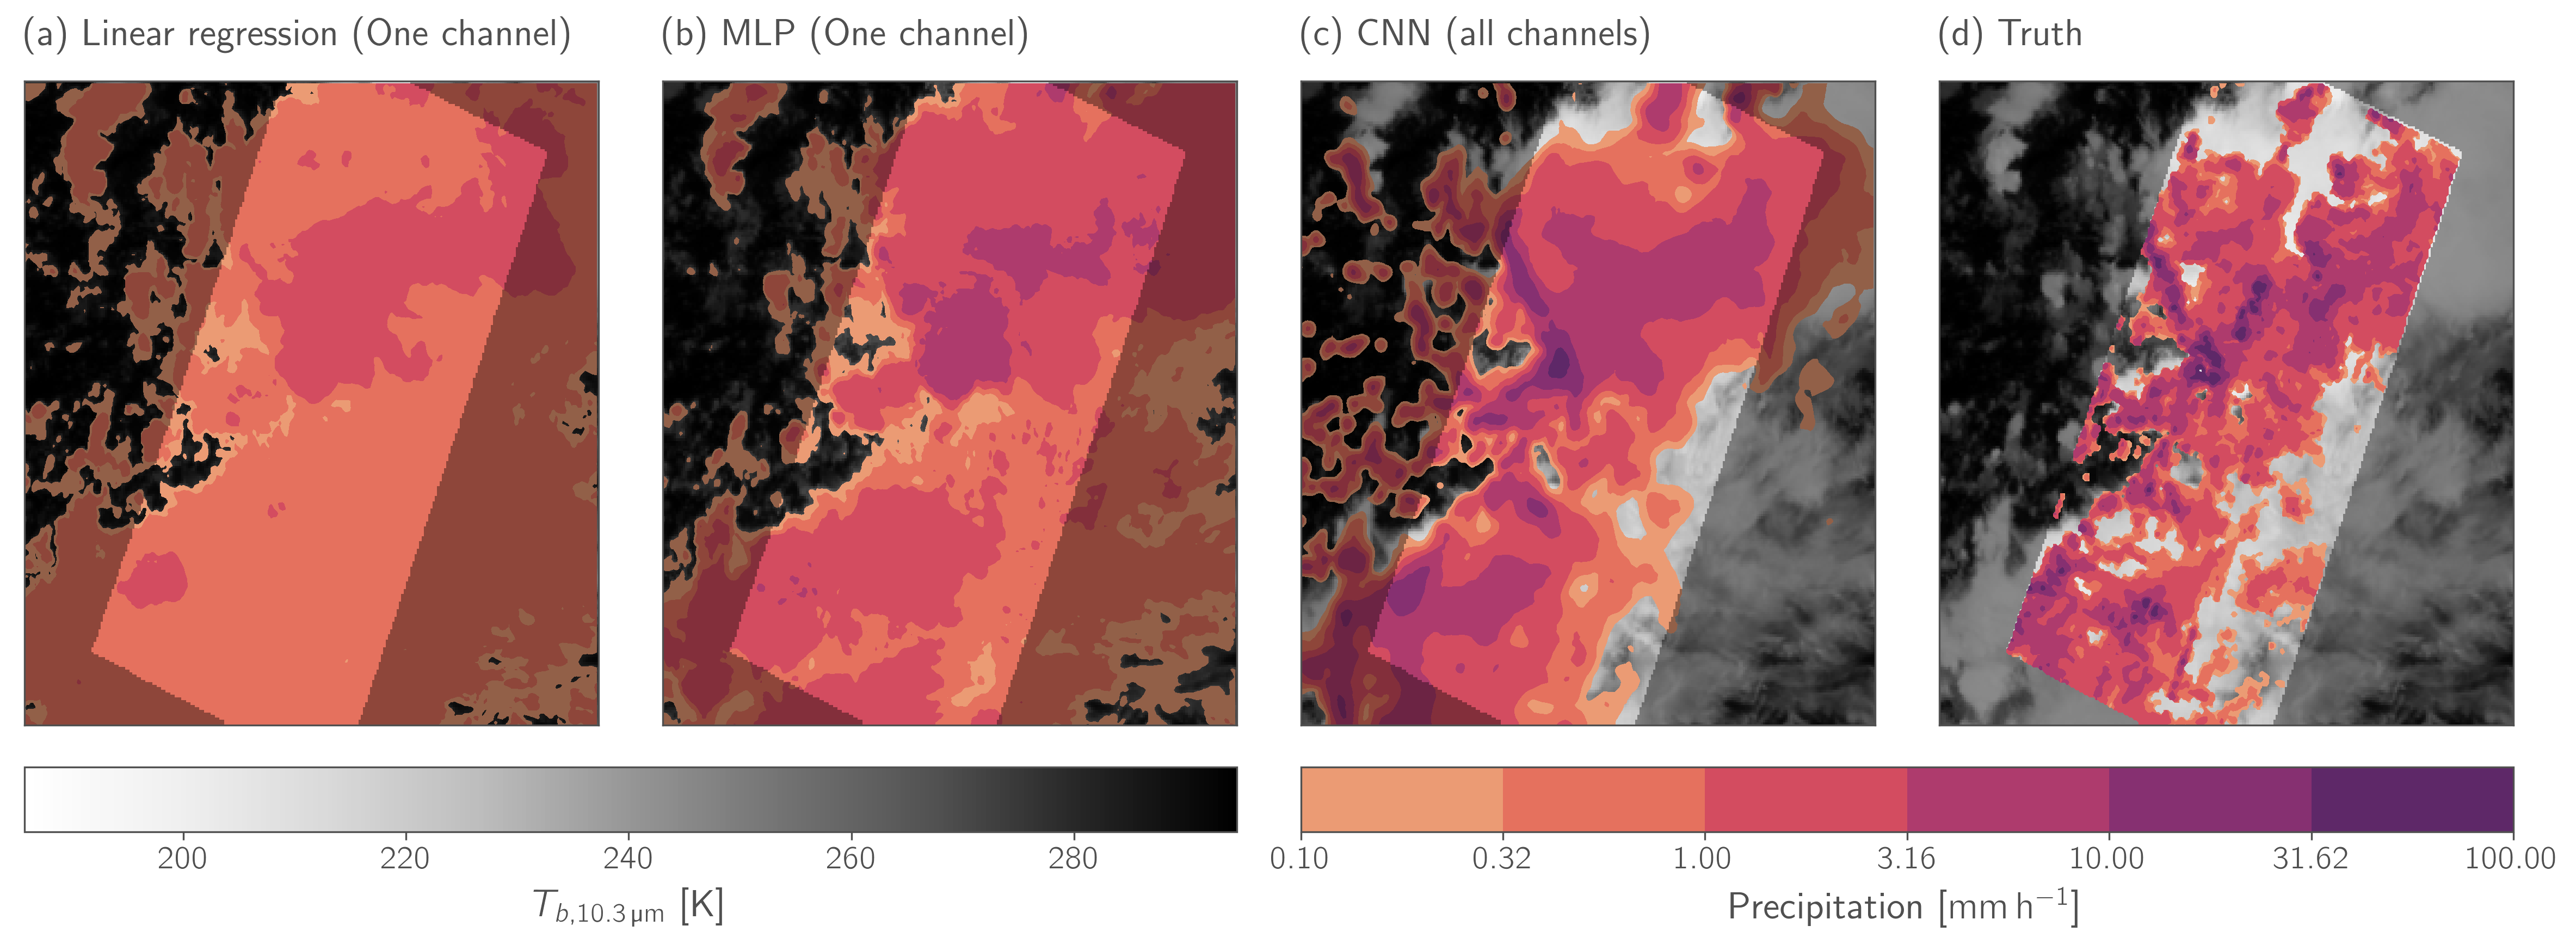
\includegraphics[width=\textwidth]{retrieval_comparison}
\caption{Retrieved precipitation from a linear regression model
  (panel (a)), an MLP applied separately to each input pixel
  (panel (b)) and a CNN that predicts precipitation for the
  full input image using all available channels (panel (c)).
  The reference precipitation measured by the combined radar
  and passive microwave retrievals of the GPM core observatory
  are shown in panel (d).}
\label{fig:machine_learning:retrieval_comparison}
\end{figure}

This example clearly demonstrates the ability of deep learning techniques to
improve remote sensing retrievals. However, it should also be noted that the
computational effort required to train these models increases by orders of
magnitude. The simple linear regression model used here takes at most a few
seconds to train. The training of the MLP and CNN models, on the other hand,
takes hours respectively days and uses dedicated computing hardware. This is in
general not an issue because the training is a one-time effort and the
evaluation of the model is much faster, but nonetheless a fact that deserves
consideration.

The results in Fig.~\ref{fig:machine_learning:retrieval_comparison} show that
even the more advanced retrieval model fails to truthfully reproduce the
precipitation in the reference data. Since VIS and IR observations from
geostationary satellites are only sensitive to the upper parts of the clouds,
the inputs provided to the retrieval are only indirectly related to
precipitation at the surface. The ill-posed character of the retrieval problem
dictates that any specific prediction from a neural network will be wrong. Given
this fundamental nature of remote sensing retrievals, the next section explores
how neural networks can learn how wrong they expect to be.


\section{Handling uncertainty in remote sensing retrievals}

One of the issues that this thesis aims to address is the quantification of
retrieval uncertainties in machine-learning-based remote sensing retrievals. The
two methods that were explored in the appended studies fall into the category of
probabilistic regression methods. This means that they account for the aleatoric
uncertainty in the prediction but neglect epistemic uncertainty and covariate
shift. Below, these two approaches are presented followed by a discussion of
other approaches for quantifying uncertainties in neural network predictions.

\subsection{Probabilistic regression}

Aleatoric uncertainty arises due to ambiguous samples in the training data. The
fact that these ambiguities are represented in the training data means that they
can be predicted by a suitably trained neural network model. To allow for this,
the deterministic formulation of regression, i.e. to predict a single value $y =
f(\vec{x})$, is replaced by a probabilistic formulation, which aims predict the
probability distribution $p(y|\vec{x})$ of $y$ given the input vector $\vec{x}$.

\subsubsection{Quantile regression neural networks}

%To predict a distribution $p(y|x)$ the neural network model can trained
%to predict parameters of a parametrized probability distribution and
%an optimization criterion for the training can be obtained by maximizing the
%likelihood of the training samples under the predicted distribution. Assuming
%$p(y|x)$ to be Gaussian distributed with mean $\mu = f(x)$ and constant standard
%deviation yields a training criterion equivalent to the MSE loss.

Quantile regression neural networks (QRNNs) predict the distribution
$p(y|\vec{x})$ for a scalar output $y$ using a sequence of its quantiles. Given
a fraction $\tau \in [0, 1]$, the corresponding quantile $y_\tau$ is defined as
\begin{align}
  y_\tau &= F^{-1}(\tau)
\end{align}
with $F(y) = \int_{-\infty}^y p(y|\vec{x})\ dy$ the cumulative distribution
function (CDF) of the distribution $p(y|\vec{x})$. A neural network can learn to predict a quantile
$y_\tau$ by training it to minimize the quantile loss
\begin{align}
  \mathcal{L}(y_\tau, y) &=
  \begin{cases}
    \tau  |y_\tau - y| & \text{if } y > y_\tau \\
    (1 - \tau)  |y_\tau - y| & \text{otherwise} \\
    \end{cases}
\end{align}
where $y_\tau$ is the predicted quantile and $y$ is the reference output value
from the training data. It is important to realize here  that $y$ is only
required to be an ordinary sample of the distribution $p(y|\vec{x})$ and does not
require the distribution $p(y|\vec{x})$ to be explicitly represented in the
training data.

The approach can be extended to the prediction of multiple quantiles
corresponding to a sequence of quantile fractions $\mathrm{T} = \{\tau_1,
\ldots, \tau_N\}$ by training the network to minimize the sum of the quantile
losses
\begin{align}
  \mathcal{L}_\mathrm{T}(\vec{y}_T, y) &= 
  \sum_{\tau \in \mathrm{T}} \mathcal{L}_\tau(y_\tau, y)
\end{align}
where now $\vec{y}_T = [y_{\tau_1}, \ldots, y_{\tau_N}]$ is a vector of predicted quantiles.

The basic principle of QRNNs is illustrated
Fig.~\ref{fig:machine_learning:qrnn}. To predict the distribution of a scalar
variable $y$ conditioned on a vector of inputs $\vec{x}$, QRNNs use a neural
network to transform the vector of inputs into a vector of outputs. The outputs
correspond to a sequence of quantiles, which can be used to derive a piece-wise
linear approximation of the CDF of $p(y|\vec{x})$.

\begin{figure}[btp]
  \centering
  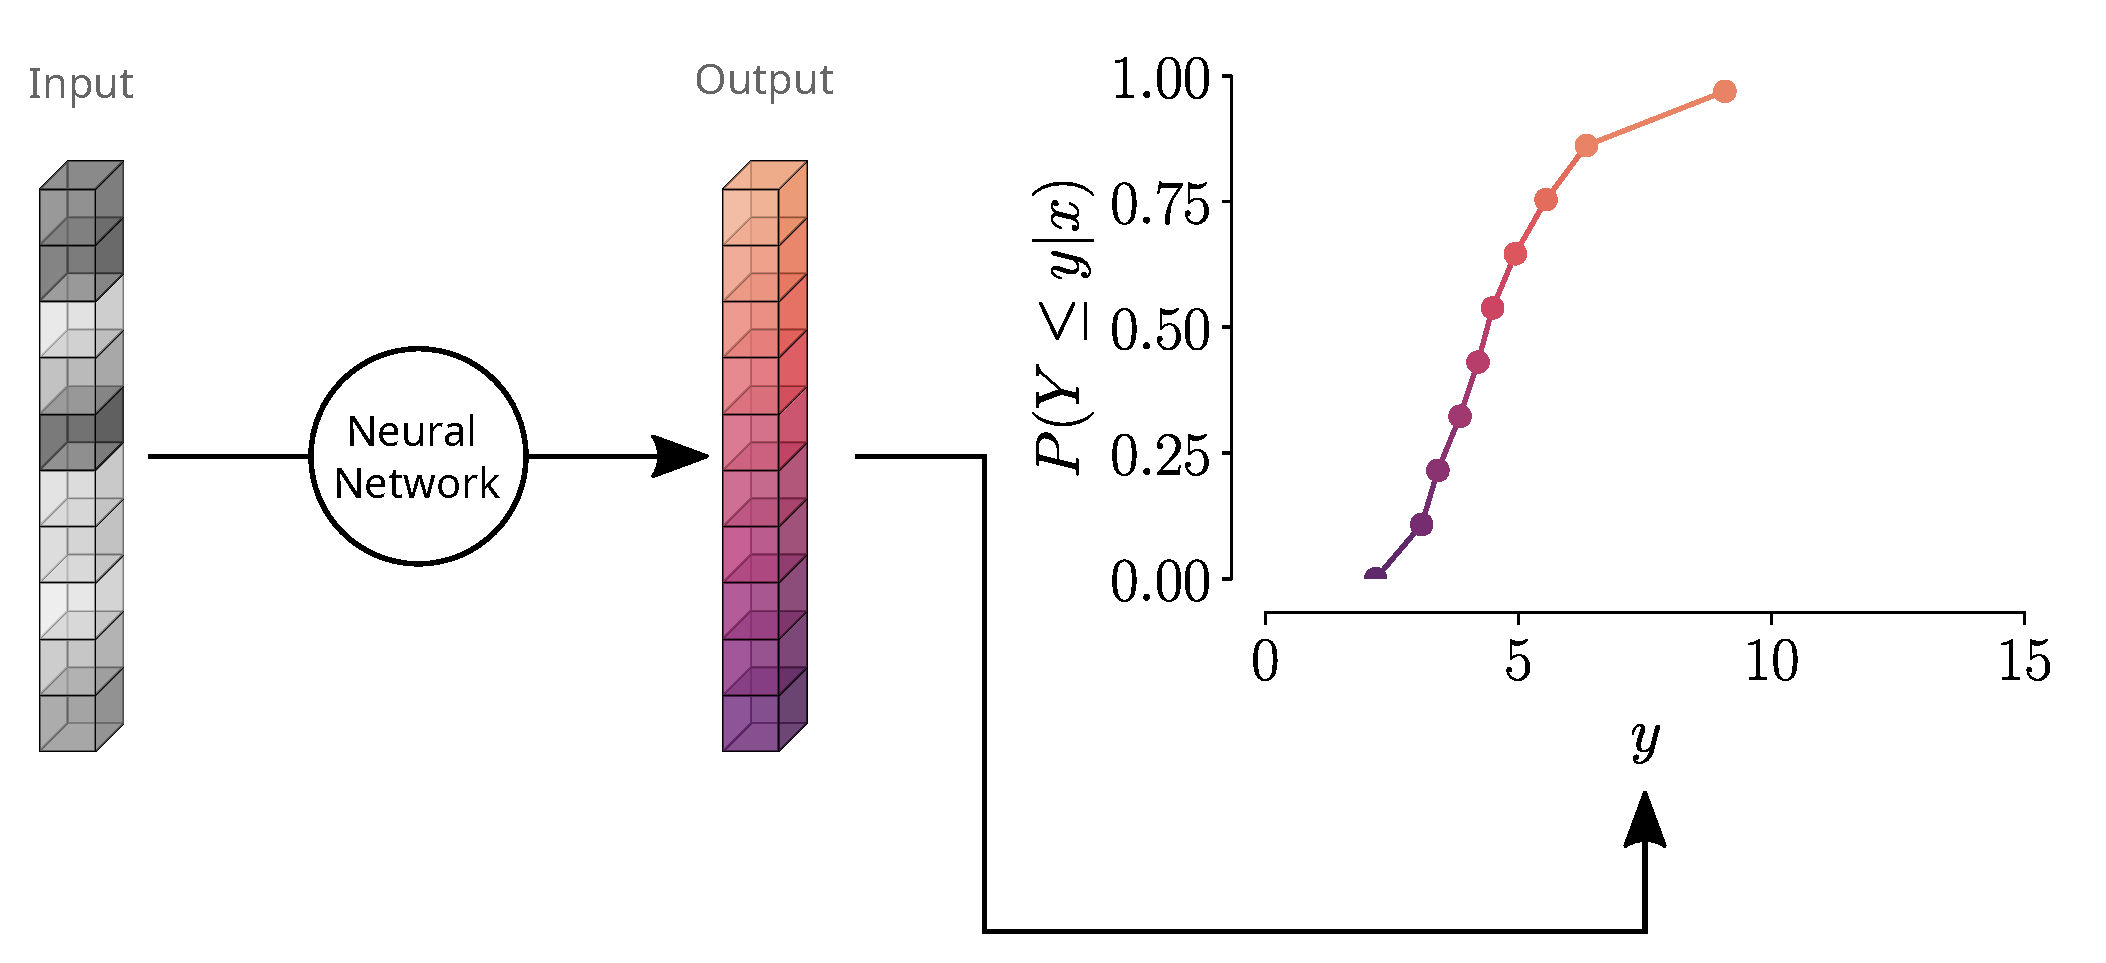
\includegraphics[width=.75\textwidth]{qrnn.pdf}
  \caption{Basic principle of QRNNS. QRNNs predict the distribution of
    a scalar output variable $y$ using a vector of quantiles from which the
    an approximation of the CDF of the distribution can be constructed.}
  \label{fig:machine_learning:qrnn}
\end{figure}

Using quantiles to represent the distribution $p(y|\vec{x})$ has the advantage
that the neural network can learn the shape of the posterior distribution of the
retrieval. This is in contrast to other probabilistic regression methods, which
often impose a more constrained parametrized form of $p(y|x)$, such as a Gaussian
whose mean and standard deviation are predicted.

An unresolved issue with QRNNs is quantile crossing. There is nothing that
ensures that the quantiles predicted by a QRNN as they are employed here are in
increasing order. QRNNs can thus produce mathematically inconsistent
predictions, where quantiles of lower fractions exceed those of higher
fractions. However, at least for the applications considered in this thesis,
this was not found to be a critical issue.

\subsubsection{Density regression neural networks}

The second approach for predicting the distribution $p(y|\vec{x})$ is based on
the work by \citet{oord16} and \citet{sonderby20}. Since it has not been given
an explicit name by the authors, it is referred to here as density regression
neural networks (DRNNs). In this approach, the regression problem is cast as a
classification problem by discretizing the domain of output values $y$ into bins
$y_0, \ldots, y_n$ and then predicting for each bin the probability $p_i(y >=
y_{i - 1}, y < y_i)$ of the observed $y$ falling into the $i$th bin.

Mathematically this is implemented by minimizing the
categorical cross-entropy loss
\begin{align}
  \mathcal{L}(\hat{\vec{p}}, y) &=  -\log(\hat{p}_i) \text { with i such that } y_{i - 1} \leq y < y_i.
\end{align}
where $\hat{\vec{p}} = [\hat{p}_1, \ldots, \hat{p}_n]$ is a vector of predicted probabilities.

The predicted vector of bin probabilities can then be used as a piece-wise
constant approximation of the PDF of $p(y | \vec{x})$, as illustrated in
Fig.~\ref{fig:machine_learning:drnn}. Since the CDF of $p(y | \vec{x})$ can be
calculated from the PDF and vise versa, QRNNs and DRNNs are functionally very
similar. Compared to QRNNs, DRNNs have the advantage of avoiding quantile
crossing by construction. What may be a disadvantage of DRNNs is that they require
a relatively high number of outputs  when the values of $y$ vary across a wide
range.
\begin{figure}[btp]
  \centering
  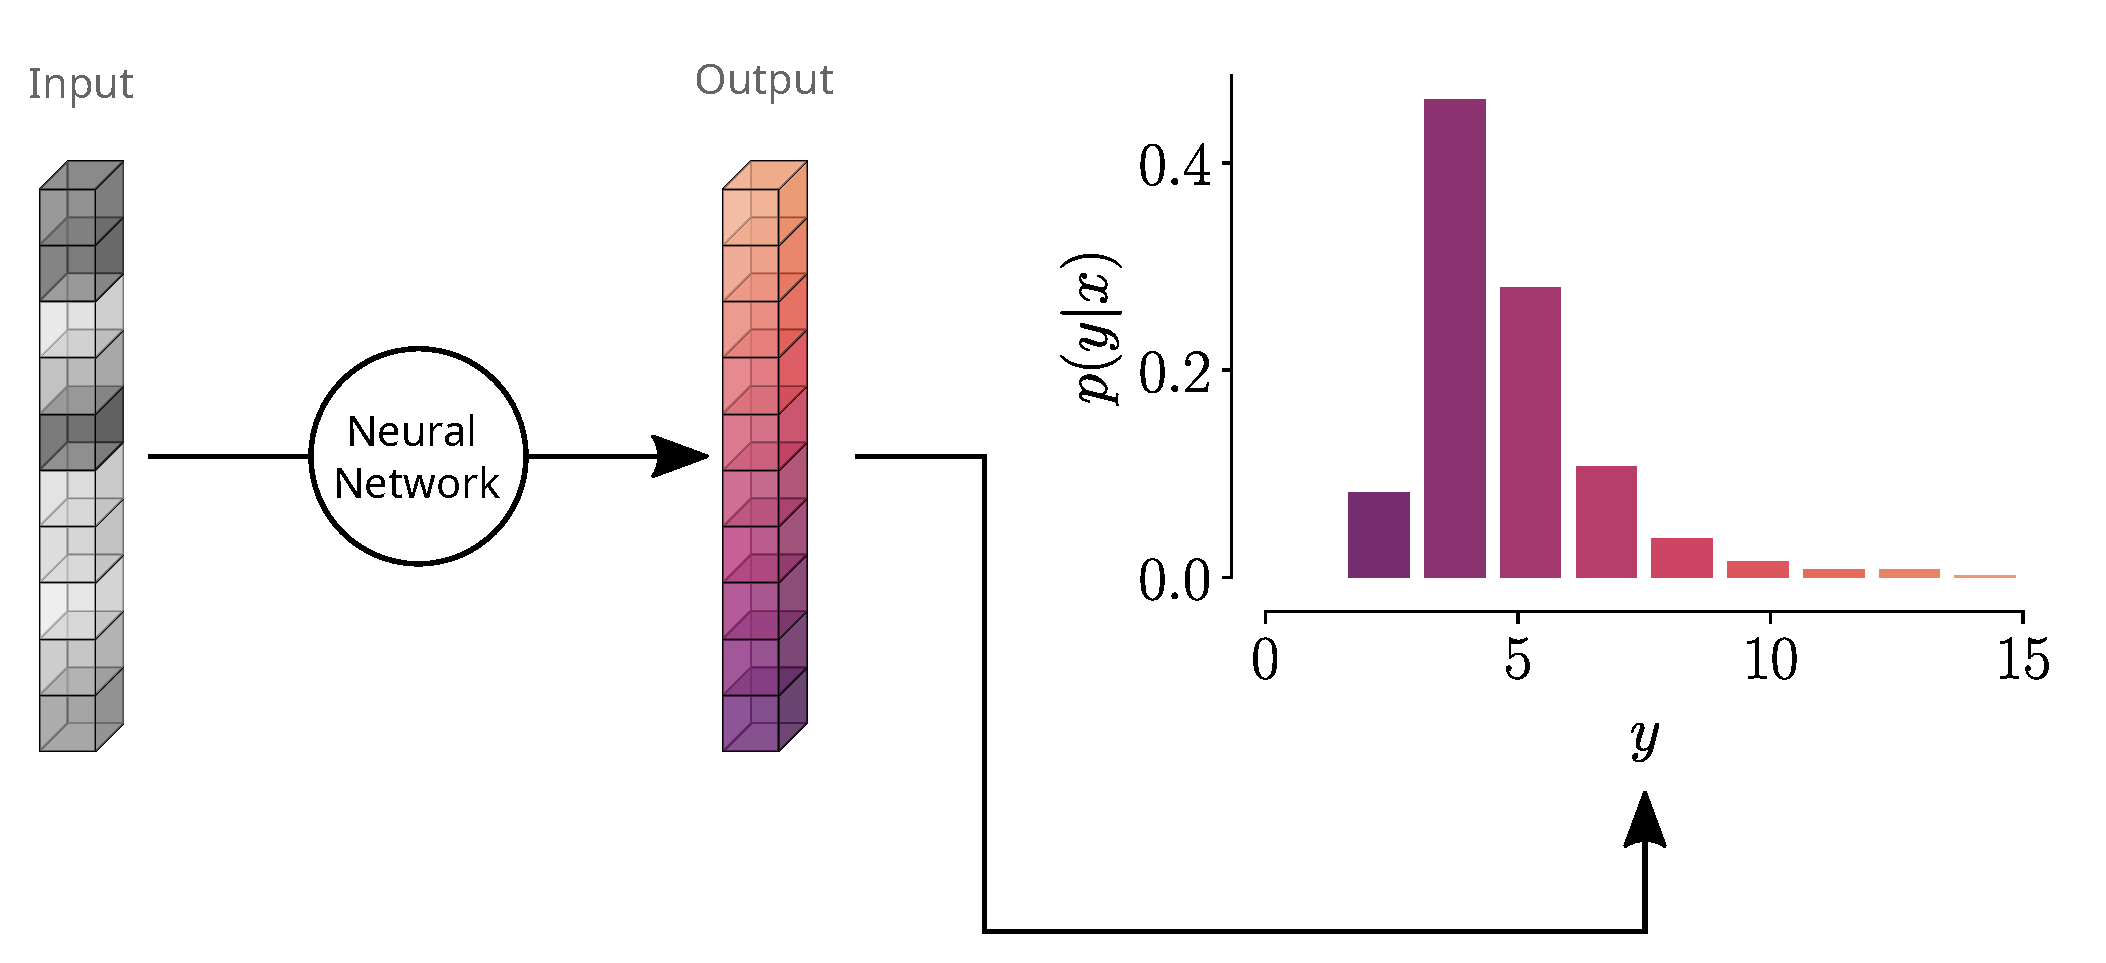
\includegraphics[width=.75\textwidth]{drnn.pdf}
  \caption{The basic functioning of QRNNS. QRNNs predict the distribution of
    a scalar output variable $y$ using a vector of quantiles from which the
    an approximation of the CDF of the distribution can be constructed.}
  \label{fig:machine_learning:drnn}
\end{figure}

\subsubsection{The aleatoric approximation}

Both QRNNs and DRNNs only learn to quantify the aleatoric uncertainty and
neglect epistemic uncertainty and covariate shift. It is thus necessary that the
aleatoric component of the predictive uncertainty dominates the two other types
of uncertainties for these models to produce reliable uncertainty estimates.
Given that remote sensing observations are produced in a controlled environment
and the range of possible observations is generally well understood, it is
usually possible to obtain large amounts of reliable training data, which
minimizes epistemic uncertainty and the effects of covariate shift. Given the
cost of designing and operating these observation systems, one should expect
that an effort is made to minimize both epistemic uncertainty and covariate
shift, thus leaving the aleatoric uncertainty as the only irreducible source of
uncertainty in the measurements. Additional, empirical evidence for the
usefulness of the aleatoric approximation comes from the results presented in
this thesis, where the probabilistic predictions from QRNNs and DRNNs were found
to provide reliable estimates of the retrieval uncertainty.

\subsubsection{Further limitations}

A further limitation of QRNNs and DRNNs is their handling of multiple retrieval
outputs. The formulations presented above were based on the assumption of a
scalar retrieval output $y$. These approaches can easily be extended to multiple
output variables by simply minimizing the mean of their individual losses. This
was found to work well in practice but provides no way of representing the
correlations between the multiple outputs in the results. QRNNs and DRNNs are
therefore not able to produce random samples  that accurately the correlations
between the output variables.

\subsection{Other approaches for quantifying uncertainties}

Because of their limitations, QRNNs and DRNNs may not be the best choice for all
applications. Therefore, the following section briefly reviews other approaches
for quantifying retrieval uncertainty and compares them to the probabilistic
regression approach.

\subsubsection{Bayesian neural networks}

Bayesian neural networks (BNNs) can handle both epistemic and aleatoric
uncertainty. For BNNs, not only the target $y$ is assumed to be a random
variable, but also the parameters $\vec{\theta}$ of the neural network model. The
random distribution of these parameters represents the uncertainty caused by the
limited amount of training data that the model is trained on. Instead of
learning specific parameters, a BNN learns a distribution of each of its
parameters.

A single prediction from a BNN $p(y|\vec{x}, \vec{\theta})$ for a specific input
$\vec{x}$ is obtained by sampling values of the model parameters from the learned
distributions and using them to evaluate the model. The epistemic uncertainty in
the model predictions is typically quantified by sampling multiple instances of
the model parameters $\vec{\theta}$ and evaluating the model for each of them. For
inputs $\vec{x}$ that the model has encountered often during training, the
distribution of $\vec{\theta}$ values will be sharp so that the distribution
$p(y|\vec{x}, \vec{\theta})$ does not change much for different realizations
of the model parameters $\vec{\theta}$. For
samples where this is not the case, there will be a larger spread and thus
higher epistemic uncertainty in the predictions.

Despite their ability to quantify both aleatoric and epistemic uncertainty, BNNs
have not yet found widespread adoption in practical applications. One reason for
this is likely that their training takes significantly more time. Another
disadvantage is that the quantification of epistemic uncertainty requires
evaluating the network multiple times. This typically increases the time
required to evaluate the model by an order of magnitude, which is a
disadvantage for applications that require high throughput.

Despite these potential disadvantages, \citet{orescanin22} have recently
demonstrated the application of Bayesian neural networks to the classification
of precipitation types and shown that the predicted uncertainties are
well-calibrated. They also found that the predictive uncertainty is dominated by
aleatoric uncertainty, which provides further evidence for the validity of
the aleatoric approximation.

\subsubsection{Generative models}

Generative models are another approach for quantifying uncertainties in neural
network predictions. Instead of predicting the conditional probability
distribution $p(\vec{y}|\vec{x})$ explicitly, these methods are trained to generate
samples from the distribution directly. These methods have gained popularity in
computer vision tasks due to their ability to generate samples from highly
complex probability distributions such as images of faces or generic objects.

The advantage of this approach is that it can handle spatial correlations in the
uncertainties, which is not the case for the other methods discussed so far.
This means that they can produce spatially coherent samples of the retrieved
variables that look very realistic. Recent work has explored the application of
generative models for short-term weather forecasting \citep{ravuri21} and
probabilistic downscaling of precipitation \citep{harris22, leinonen20}.
However, these models are also known to be more difficult and take longer to
train. In addition to that, they also need to be evaluated multiple times to
calculate statistics of the posterior distribution, which increases the
computational requirements of the retrieval.


\chapter{Contributions}

The previous chapter introduced QRNNs and DRNNs as machine-learning-based
methods to perform remote sensing retrievals. The motivation for this was to
find a practical approach to combine the capabilities of modern deep neural
networks with the theoretically sound handling of uncertainties of conventional,
inverse-theory-based retrieval methods. To explore the validity and practicality
of the proposed methods, they have been applied to idealized scenarios and
multiple real-world retrieval applications. This section presents this work and
summarizes the main results.

\section{Handling retrieval uncertainty with neural networks}

The first of the appended papers, entitled \textit{A neural network approach to
estimating a posteriori distributions of Bayesian retrieval problems} and
published as \citet{pfreundschuh18}, proposes using  QRNNs for remote
sensing retrievals. The study was motivated by the shortcomings of the
retrieval methods that were available at the time of its writing. The Bayesian
framework provides a principled way of handling uncertainties in remote
sensing retrievals (see Sec.~\ref{sec:machine_learning:retrieval_problem}),
but the commonly used methods are computationally complex. While retrievals
based on neural networks were already common and often offered superior
performance in terms of computational cost as well as accuracy, the retrieval
uncertainties were typically neglected.

The aims of the study are two-fold: (1) to demonstrate the compatibility of
QRNNs with conventional Bayesian retrieval methods and (2) to demonstrate the
practicality of QRNNs by applying them to a real-world retrieval application.

An idealized but realistic retrieval scenario in which the full Bayesian
solution could be calculated to arbitrary precision was designed to demonstrate
the compatibility of QRNNs with conventional Bayesian retrieval methods. The
study applies QRNNs and Bayesian Monte Carlo Integration (BMCI), a commonly used
Bayesian retrieval method, to solve the retrieval and compares their solutions
to the true solution. BMCI calculates an approximate solution of the retrieval
problem using a database of observations and corresponding reference values.
This makes it similar in this regard to machine learning methods. The results
show that QRNNs work at least as well as BMCI in solving the retrieval problem,
given that both are based on a sufficiently large dataset. There is a clearer
advantage for QRNNs for smaller datasets, indicating that they cope better with
the curse of dimensionality.

This first result has two important implications. Firstly, it showed that QRNNs
can be used instead of BMCI and expected to work at least as good given the same
training data. Even if the advantage of neural networks over BMCI on the
considered dataset was marginal when sufficient training data is available, the
use of neural networks offers distinct advantages compared to BMCI. For one, the
time required to produce a neural network prediction is independent of the
training data size. At least for a naive implementation of BMCI this time scales
linearly with the size of the training database. This means that the amount data
that can be used by the method may be limited by operational processing
requirements. Besides that, because of the flexibility of QRNNs, they can be
easily extended to image or time-series data, which is not as simple for BMCI or
other Bayesian retrieval methods.

The second important implication of these results is that they show the
compatibility of probabilistic machine learning methods with Bayesian retrieval
methods. These results link the extensive theory on Bayesian retrievals
\citep{rodgers00, tarantola05} with machine-learning-based methods. In
particular, the correspondence between the training data of the neural network
and the a priori distribution of a Bayesian retrieval highlights their
importance for accurate quantification of retrieval uncertainties.


%Two experiments were performed in the study. The first one used an idealized
%retrieval scenario in which samples from the posterior distribution $p(y|x)$
%could be calculated using Markov Chain Monte Carlo (MCMC) methods. MCMC is
%generally too slow to be used in operational processing, but its ability to
%generate samples from the true posterior distribution makes it suitable to
%provide a reference solution against which QRNNs and another Bayesian retrieval
%method could be evaluated. A principal results from this experiment is shown
%Fig.~\ref{fig:contributions:cdfs_qrnn_bmci}. The plot displays the retrieved
%CDFs of the posterior distributions using QRNN and Bayesian Monte Carlo
%Integration (BMCI), which is a commonly used Bayesian retrieval methods. Each
%panel shows the reference CDF obtained using MCMC in the background and the CDFs
%obtained using BMCI in blue, those obtained from a single QRNN using a solid red
%line and those obtained from an ensemble of QRNNs using red markers. The shown
%samples were chosen according to the Kolmogorov-Smirnov of the BMCI
%($\text{KS}_\text{BMCI}$) and QRNN ($\text{KS}_\text{QRNN}$), which measures
%the agreement between the reference and retrieved CDF, and thus show retrieval
%results of varying quality from each retrieval.
%
%The main finding from this first experiment is that the CDFs retrieved using
%QRNN and BMCI agree very well with the reference CDF calculated using MCMC. This
%indicates that probabilistic neural network retrievals are consistent with the
%Bayesian solution of inverse problems with the a priori distribution being
%represented by the training data.
%
%\begin{figure}
%  \centering
%  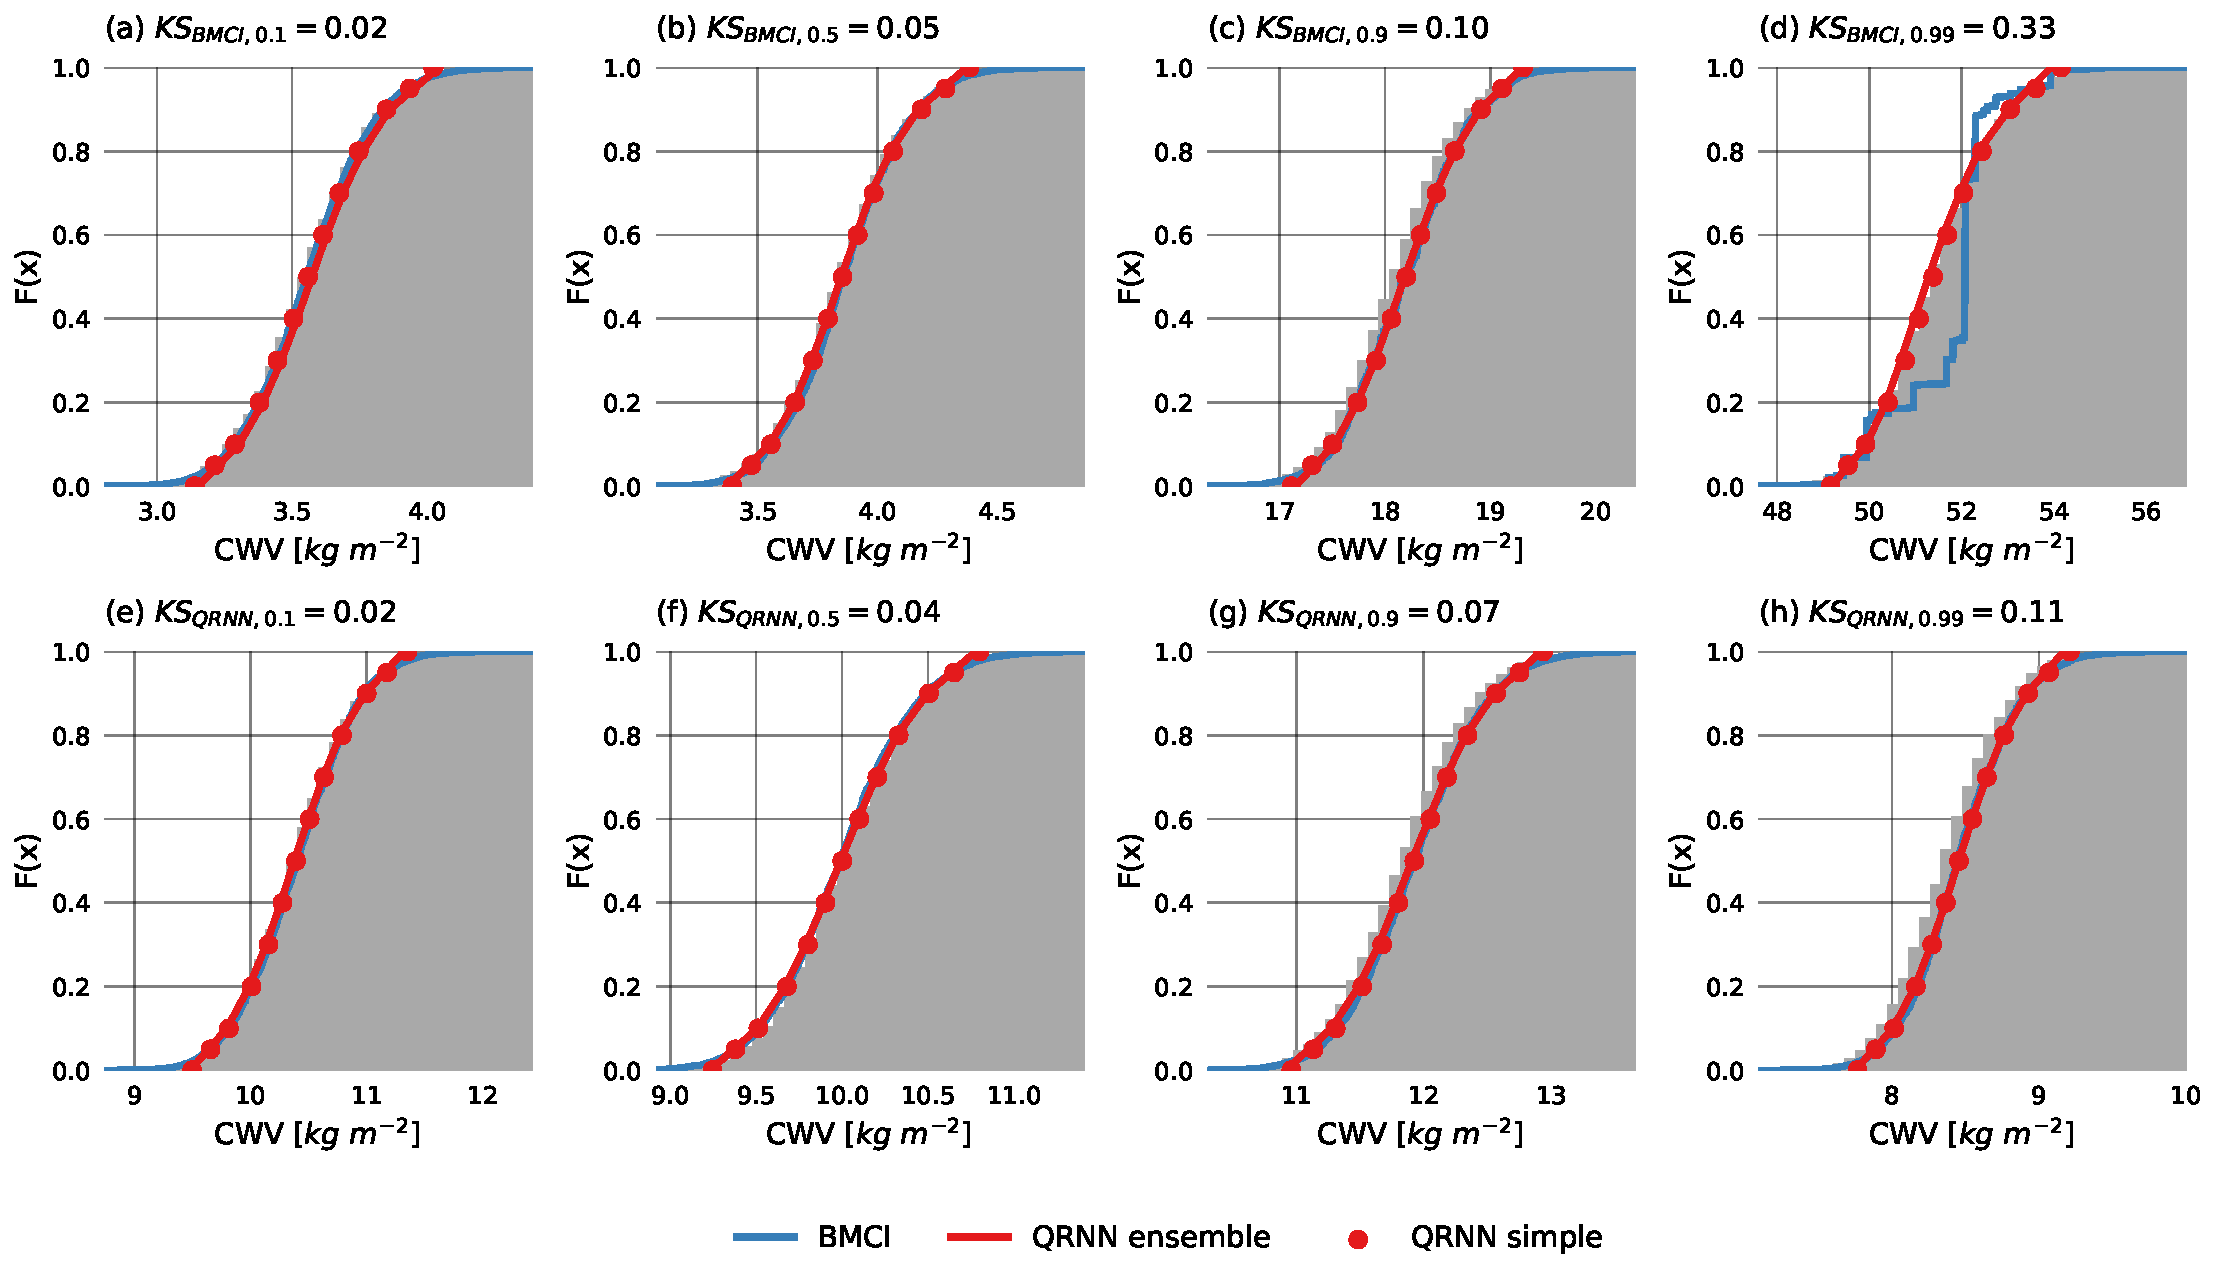
\includegraphics[width=\textwidth]{cdfs_qrnn_bmci}
%  \caption{ Retrieved a posteriori CDFs obtained using MCMC (gray), BMCI (blue),
%    a single QRNN (red line) and an ensemble of QRNNs (red marker). Cases
%    displayed in the first row correspond to the 1st, 50th, 90th and 99th
%    percentiles of the distribution of the Kolmogorov– Smirnov statistic of BMCI
%    compared to the MCMC reference. The second row displays the same percentiles
%    of the distribution of the Kolmogorov–Smirnov statistic of the single-QRNN
%    predictions compared to MCMC.}
%  \label{fig:contributions:cdfs_qrnn_bmci}
%\end{figure}

The second experiment from this study applied QRNNs to the retrieval of cloud
top pressure (CTP) from infrared observations from the Moderate Resolution
Imaging Spectroradiometer (MODIS). The comparison of the QRNN retrieval to an
existing algorithm based on a deterministic neural network shows that QRNNs
yield comparable or better accuracy for point predictions with the added benefit
of providing reliable uncertainty estimates.

A principal result from this experiment is shown in
Fig.~\ref{fig:contributions:qrnn_errors}, which shows the predicted and observed
distributions of retrieval errors for QRNNs as well as for the deterministic
retrieval combined with a Gaussian error model fitted on the test data. As the
comparison of the distribution shows, the Gaussian error model does not provide
a good description of the retrieval error, whereas the QRNN successfully
predicts its distribution. This results shows the ability of the QRNN to
represent non-Gaussian retrieval errors and the superiority over commonly
assumed Gaussian error models. A consequence of these findings was the adoption
of QRNNs for the operational production of near-real-time retrievals of cloud
top pressure at the European Organisation for the Exploitation of Meteorological
Satellites.

\begin{figure}
  \centering
  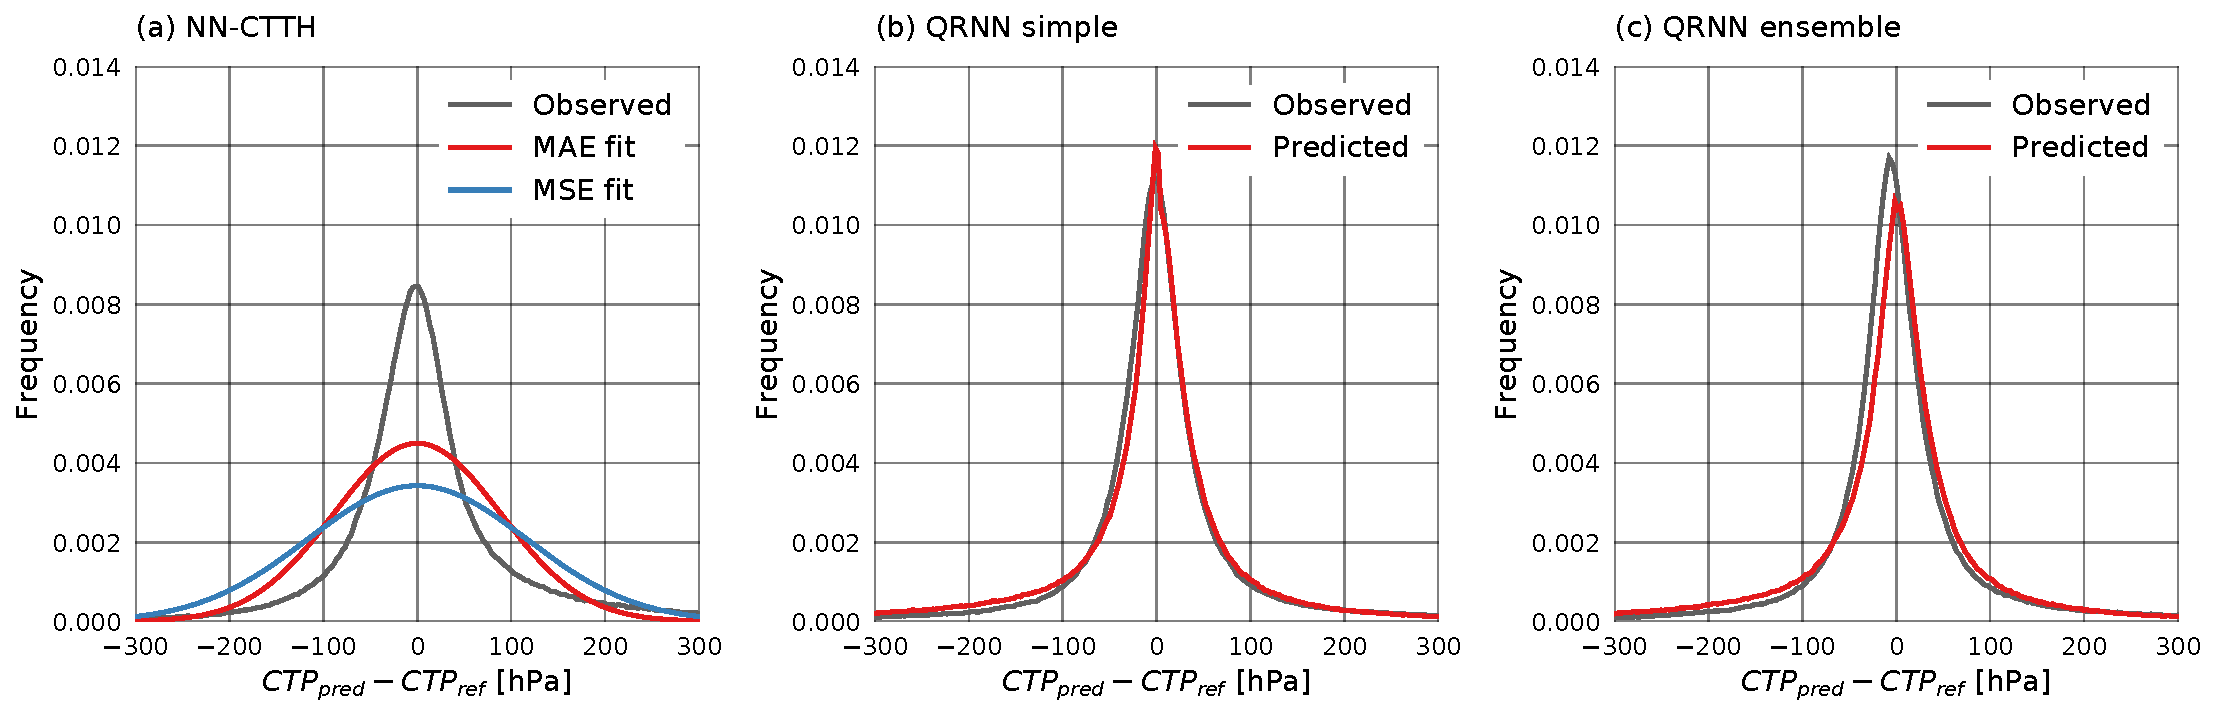
\includegraphics[width=0.75\textwidth]{qrnn_predicted_errors}
  \caption{Distributions of predicted and observed cloud-top pressure (CTP)
    retrieval errors. Panel (a) shows the results for a deterministic neural
    network combined with a Gaussian error models fitted used the mean squared
    error (blue) and the mean absolute error. Panel (b) show the
    corresponding results for the QRNN retrieval.}
  \label{fig:contributions:qrnn_errors}
\end{figure}

\section{Passive microwave precipitation retrievals}

The second study included in this thesis, entitled \textit{ GPROF-NN: A neural
  network based implementation of the Goddard Profiling Algorithm} and published
as \citet{pfreundschuh22a}, applied the QRNN methodology to the retrieval of
precipitation from passive microwave (PMW) observations of the GPM mission (see
Sec.\ref{sec:radiative_transfer:synergies}). GPM is an international satellite
mission lead by NASA and JAXA, which aims to provide global measurements of
precipitation at high spatial and temporal resolution.

 %The mission is built around the Core Observatory satellite, which carries a
 % precipitation radar and a PMW sensor dedicated to the remote sensing of
 % precipitation. Retrievals from the combined radar/PMW observations from the
 % Core Observatory are used to build a retrieval database that is in turn used
 % to for the retrievals of a constellation PMW sensors. As of this writing, the
 % GPM constellation comprises 9 active satellites.

The algorithm that is used to retrieve precipitation from GMI, the PMW
sensor on the GPM core observatory, and the other PMW sensors of the GPM
constellation is the Goddard Profiling Algorithm (GPROF,
\citeauthor{kummerow15}, \citeyear{kummerow15}). GPROF is based on the BMCI
method and retrieves surface precipitation as well as profiles of hydrometeor
concentrations and latent heating rates. The aim of the study was to assess the
potential benefits of replacing BMCI with a neural-network-based retrieval.
Besides that, it aims to explore to what extent the accuracy can be improved if
spatial information is incorporated into the retrieval instead of processing
each pixel separately as the current implementation does. To this end, two
neural-network-based implementations were developed. The first one, named
GPROF-NN 1D, uses an MLP to retrieve precipitation from a single pixel. The
second one, GPROF-NN 3D, uses a CNN to retrieve precipitation using  the full
swath of observations. This allows the GPROF-NN 3D retrieval to leverage
structural information in the observations, which is not available to the two
other implementations.

Both the GPROF-NN 1D and GPROF-NN 3D retrieval were developed to be functionally
equivalent to the currently operational GPROF algorithm so that they can
potentially replace it in an upcoming update. Moreover, the implementations were
restricted to use exactly the same data for their training as the current
method, which was done to ensure that the comparison of the three methods isn't
obscured by differences in the training data.

While the application of QRNNs to the GPROF algorithm is in principle
straightforward, the requirement to develop a retrieval that uses and produces
identical in- and output data and is based on the same data as the current
implementation of GPROF proved challenging. The training data for the sensors of
the GPM constellation makes use of radiative transfer simulations. However,
these are not generated for full swaths of observations but only for single
pixels. This makes the simulation data unsuitable for the training of CNNs.
Since extending the simulations to the full swath is currently not possible, an
intermediate CNN-based `retrieval' was trained to emulate the simulations of PMW
observations.

%proved challenging especially for the GPROF-NN 3D retrieval. The training data
%for all sensors of the GPM constellation is based on combined radar/radiometer
%observations from the GPM satellite. Since these observations are only available
%at a $\SI{100}{\kilo \meter}$-wide swath at the center of the GMI observations,
%a way had to be found to extent these to the full GMI-swath and to remap them to
%the viewing geometries of the other sensors. The current approach uses an
%intermediate simulator network to extend the simulated observations to the full
%swath of GMI, which are then remapped to the viewing geometries of other sensors
%by interpolation. This solution should be a considered a heuristic that was
%pursued mainly because extending the simulations that are routinely performed
%for the generation of the GPROF training data would have been outside the scope
%of this study.

The main results from this study are estimates of potential improvements in
retrieval accuracy that are achievable by upgrading GPROF to either the GPROF-NN
1D or GPROF-NN 3D retrieval. Consistent improvements for the GPROF-NN 1D
algorithms are found across a range of accuracy metrics for the retrieved
surface precipitation as well as the hydrometeor profiles. The accuracy is
improved further by the GPROF-NN 3D retrieval, which yields improvements similar
in magnitude to those provided by the GPROF-NN 1D algorithm over the GPROF
baseline retrieval. Furthremore, we found that the effective resolution of the
retrieval improves by at least $\SI{40}{\percent}$ for the neural-network-based
retrievals.

An example of the improvements afforded by the neural-network-based retrievals
is shown in Fig.~\ref{fig:machine_learning:hurricane_harvey}. This plot shows
the smoothed surface precipitation from the combined retrieval from the GPM core
observatory as a reference and the retrievals from the GPROF and GPROF-NN
algorithms. The comparison shows that the GPROF-NN retrievals are spatially
better resolved and improve the agreement with the combined retrievals.

\begin{figure}
  \centering
  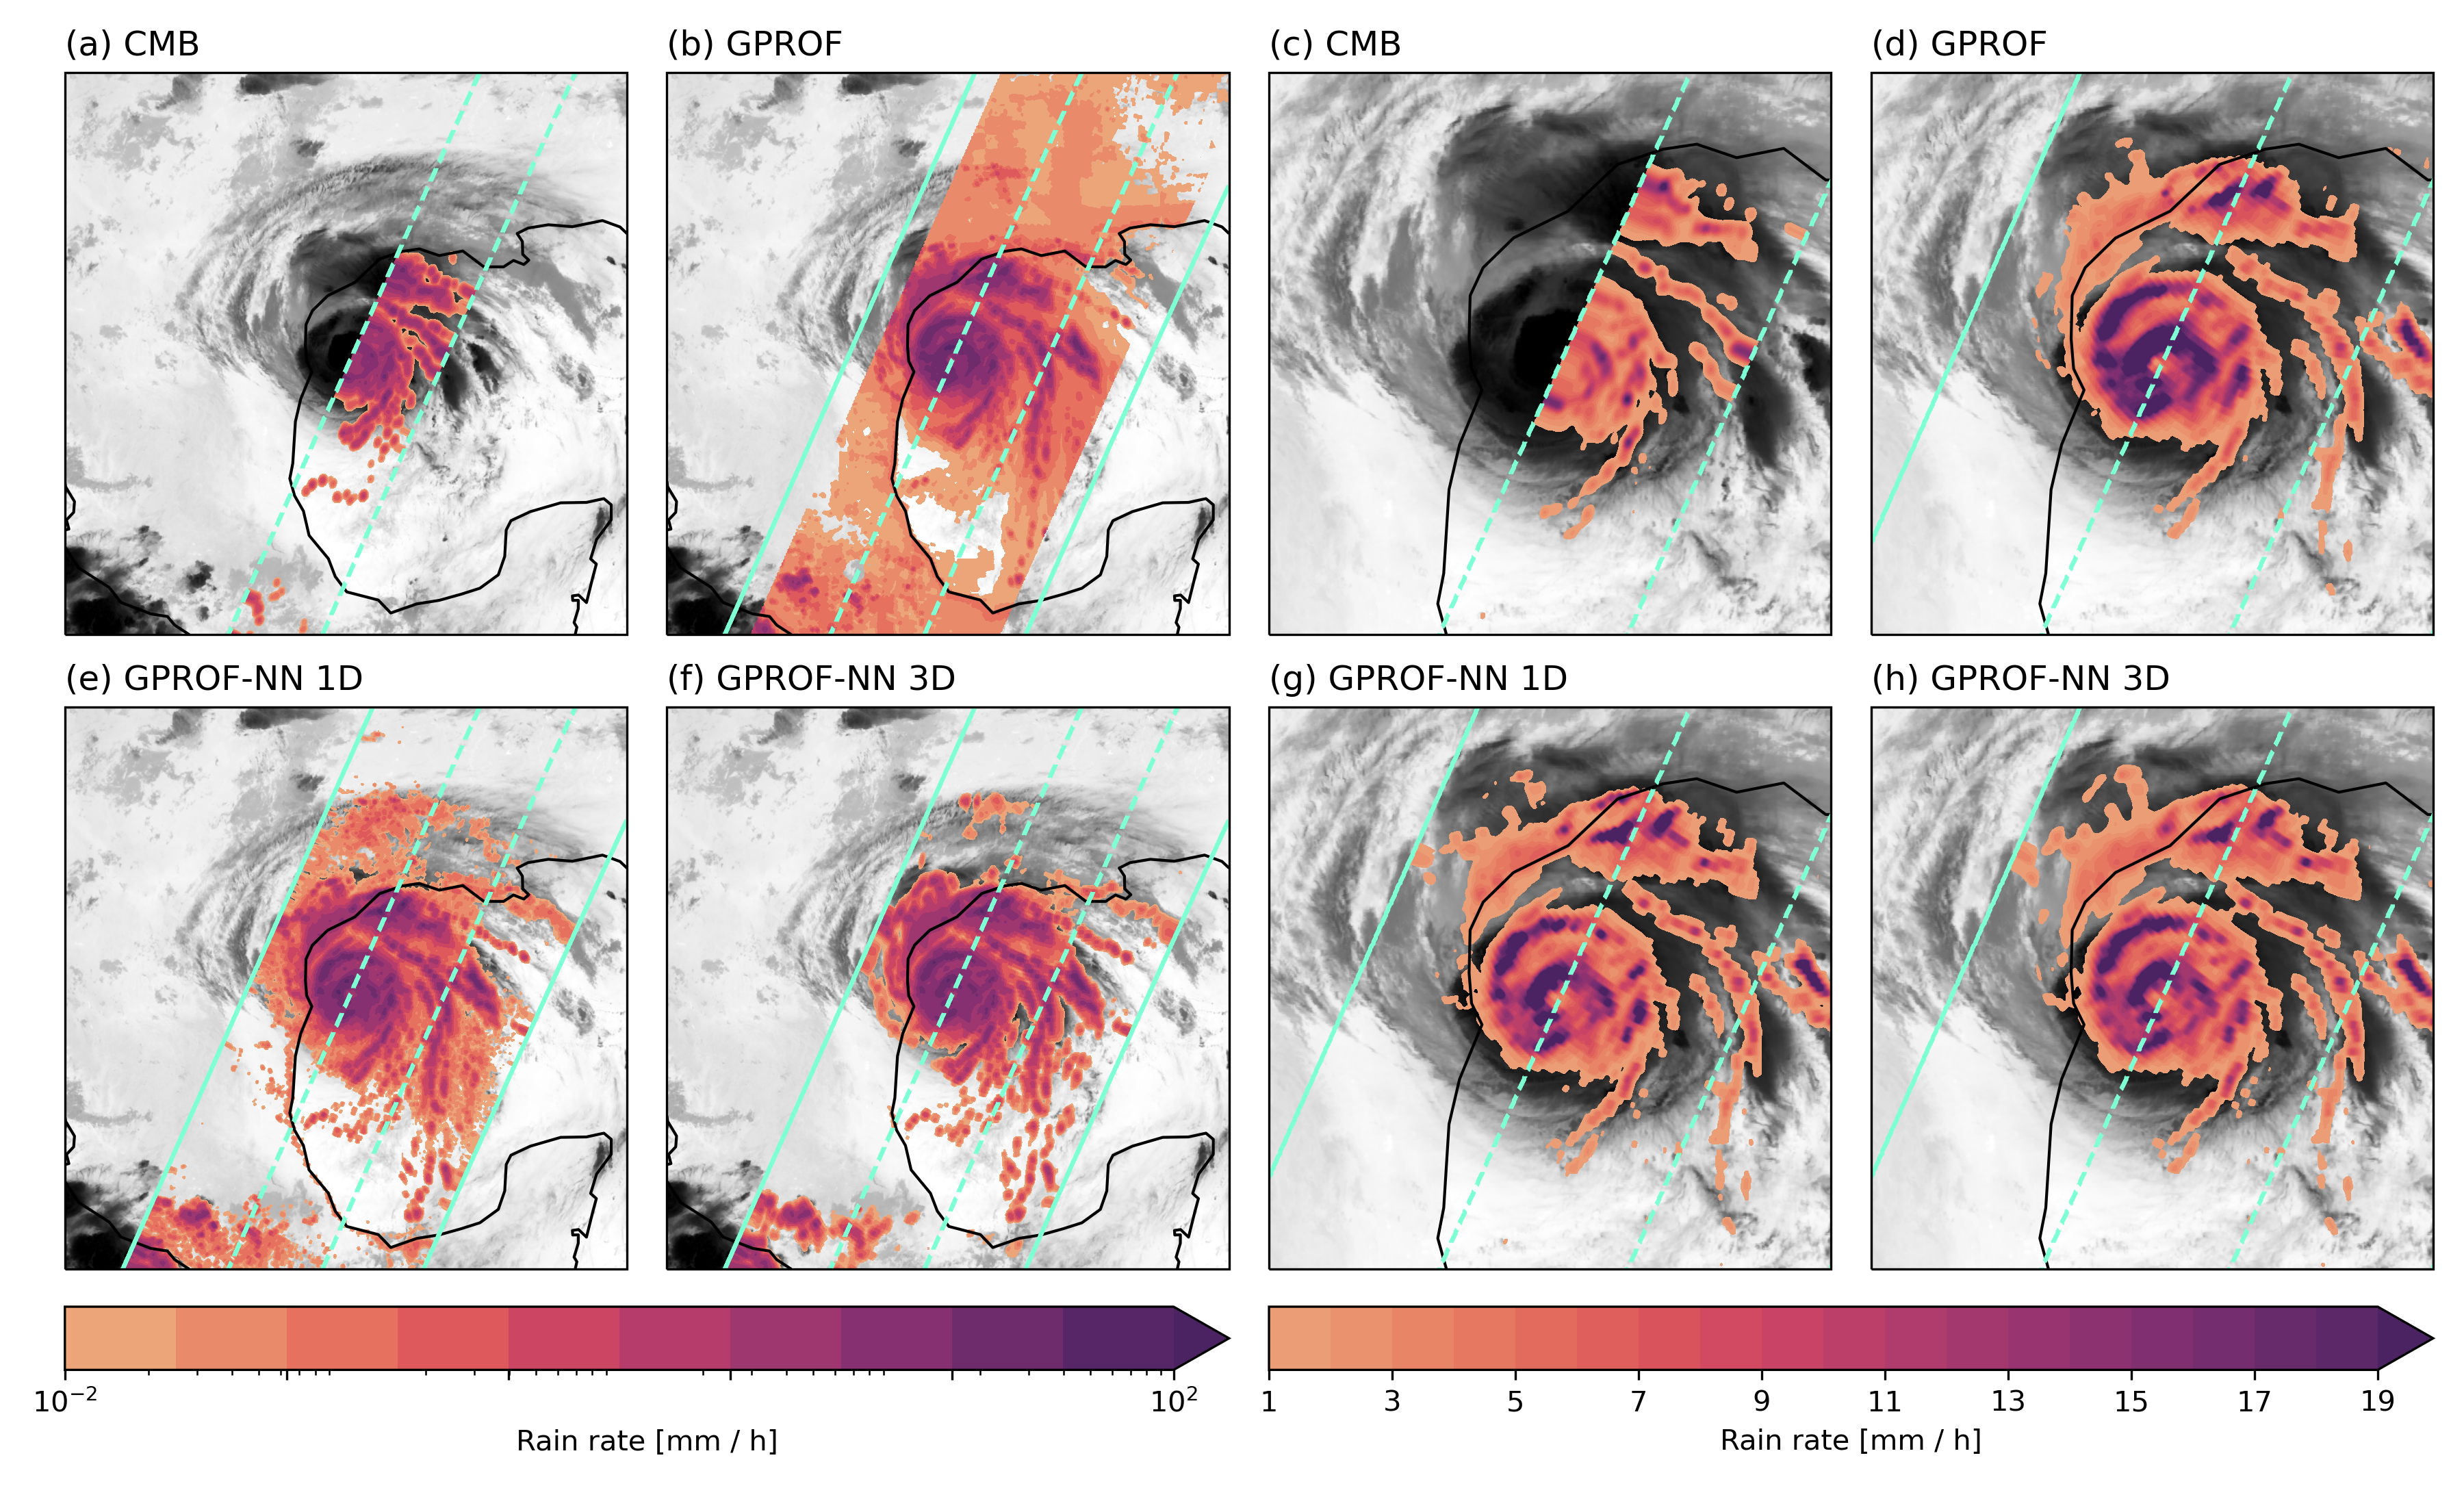
\includegraphics[width=\textwidth]{surface_precip_harvey_gmi_ir}
  \caption{ Retrieved surface precipitation from the GPM combined product
    (Panels (a), (c)), the GPROF algorithm (Panels (b), (d)), and the neural
    network versions GPROF-NN 1D (Panels (e), (g)) and GPROF-NN 3D (Panels (f),
    (h)) in and around Hurricane Harvey on 2017-08-25 at 11:50:00 UTC. Panels
    (a), (b), (e), (f) display the precipitation on a logarithmic scale over an
    area spanning $2\ 000\ \unit{km}$ in zonal and meridional directions.
    Panels (c), (d), (g), (f) display the surface precipitation on a linear
    color scale in an enlarged area spanning $500\ \unit{km}$ around the
    Hurricane. The background shows $10.3\ \unit{\mu m}$ brightness temperatures
    from the GOES 16 observations closest to the overpass.
  }
  \label{fig:machine_learning:hurricane_harvey}
\end{figure}

Although the results from this study were promising, their significance was
limited because the evaluation of the retrieval was restricted to the same
source of data that was used for the generation of the training data. Since the
objective of the study was to compare the BMCI retrieval method with QRNNs, this
simplification was justified. In a validation against independent data,
potential benefits may be obscured by deviations between training data and the
data used for validation. However, the practically more relevant question is, of
course, to what extent the neural network retrievals improve the precipitation
estimates when compared to independent validation data.

A study that addresses this question is currently under preparation and included
in this thesis as the third paper, entitled \textit{%
  Evolution of the GPROF
  passive microwave precipitation retrievals evaluated against ground radar
  measurements over the continental US and the Pacific Ocean%
}. Since the
  development of the GPROF-NN algorithms was performed in parallel with a new
  version of the GPROF retrieval, this study aimed to assess improvements in
  this new version of GPROF (GPROF V7) against the previous version (GPROF V5)
  , as well as the potential benefits of replacing GPROF with GPROF-NN 1D or 3D in
  a future update. Furthermore, the study aims to identify potential outstanding
  issues impeding the adaptation of the GPROF-NN retrievals for operational
  processing.

The validation is based on ground-radar measurements of precipitation
specifically created for the validation of GPM measurements. It is
based on measurements from the continental United States (CONUS) and a ground radar
station on the Kwajalein atoll in the Pacific Ocean.

The main focus of this study is put on retrievals from the GMI radiometer, which
plays a special role in the GPM constellation due to it being designed
specifically for the remote sensing of precipitation. The accuracy of the
precipitation retrieved from the GMI sensor using the two versions of the
conventional GPROF algorithm as well as the two GPROF-NN retrievals is evaluated
for two years of co-locations. The results clearly show that the benefits of the
neural-network-based implementation of GPROF carry over to validation against
independent precipitation measurements. In particular, the effective resolution
of the retrieved precipitation over land is improved  by more than a
factor of two.

The principal results from this study are shown in
Fig.~\ref{fig:machine_learning:gprof_nn_metrics}. The graphs show error metrics
of the retrieval when compared against the training data (labeled Database) as
well as compared against ground-based radar measurements over the period of two
years. These results clearly show that the GPROF-NN retrievals consistently
improve the instantaneous errors in the retrieval. For the biases,
the results are less obvious, but the fact that the combined retrieval
(labeled GPM-CMB) exhibits similar biases suggests that the origin for these
biases is at least in part in the training data itself.

  \begin{figure}[!hbpt]
    \centering
    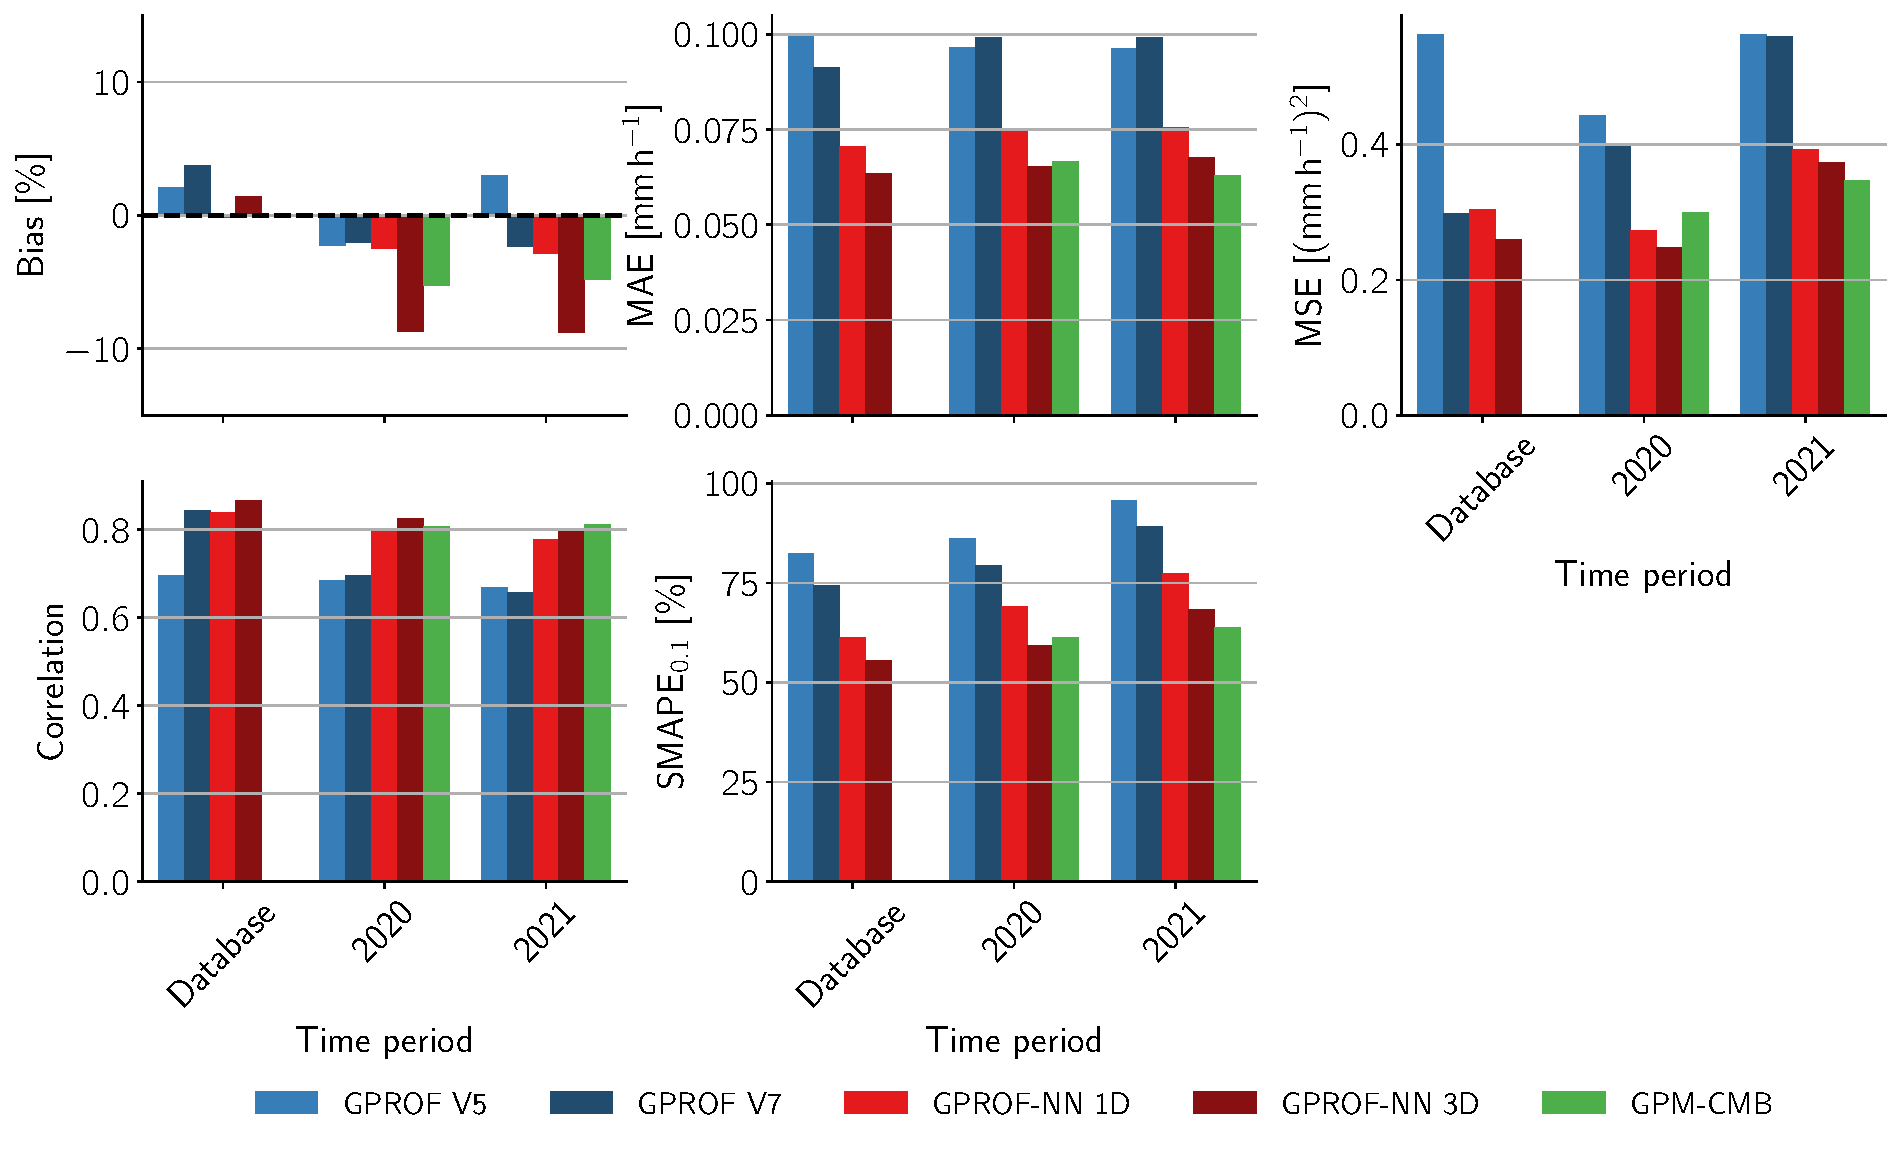
\includegraphics[width=\textwidth]{gprof_nn_metrics.pdf}
    \caption{
      Accuracy metrics of the GPROF retrievals compared to the training data
      (Database) and gauge-corrected ground-radar measurements for the water
      years 2020 and 2021.
    }
    \label{fig:machine_learning:gprof_nn_metrics}
  \end{figure}

In addition to GMI, also the retrieval accuracy of a limited number of other
sensors of the GPM constellation is evaluated. For the two sensors that have
been evaluated so far, smaller improvements in retrieval accuracy are found.
This is nonetheless an encouraging result because these sensors is affected by
errors in the radiative transfer simulation required to generate the training
data, which is not the case for the retrieval for GMI.

\section{Near real-time rain retrievals over Brazil}

While the neural-network-based implementation of GPROF provided  evidence
for the potential of neural-network-based precipitation retrievals, the
constraint of a retrieval that provides the same output as the current
operational GPROF algorithm did not leave much room to explore retrieval
improvements afforded by the probabilistic retrieval results. The two studies on
the development and assessment of the GPROF-NN retrievals presented above
therefore focused mostly on deterministic precipitation estimates and did not
explore the full potential of the probabilistic predictions afforded by the
neural networks.

The aim of the third study presented in this thesis, titled \textit{%
  An
  improved near real-time precipitation retrieval for Brazil%
} and published as
  \citet{pfreundschuh22b}, was to explore the full potential of probabilistic
  neural-network based precipitation retrievals in the context of near real-time
  retrievals from VIS and IR observations over Brazil. The input data for the
  retrieval comes from the advanced baseline imager (ABI, \citeauthor{schmit18},
  \citeyear{schmit18}) on the geostationary operational environmental satellite
  (GOES) 16. The input observations were co-located with
  retrievals from the combined radar and passive microwave observations
  from the GPM Core Observatory to generate the training data.

%The disadvantage of the observations of the ABI for precipitation retrievals is
%that they are limited to the VIS and IR regions and therefore only provide only
%indirect information on surface precipitation. However, their ability to provide
%observations every $\SI{10}{\minute}$ over Brazil and their very high spatial
%resolution still justifies their application for precipitation near real-time
%precipitation retrievals.

To validate the neural-network-based retrievals, their results were compared to
one month of gauge measurements. The retrieval accuracy was assessed by
comparing it to the retrieval algorithm that is currently used operationally at
the Brazilian National Institute of Space Research as well as two other
commonly used, global precipitation retrievals. This comparison shows that,
despite the limited information content of VIS/IR observations,
deep-learning-based retrievals outperform currently available methods, even
those that merge IR observations from geostationary satellites with passive
microwave observations.

Assessment of the predicted uncertainties against the gauge measurements shows
that they are reliable, given that differences between training  and reference
 data are taken into account. In addition to that, the study presented ways
of leveraging probabilistic retrieval results to improve the characterization of
precipitation. The predicted uncertainties can be used, for example, to derive
the probability of the observed rain exceeding a given threshold. When the
probabilistic prediction are used in this way, the retrieval  outperforms
all reference retrievals for the detection of heavy precipitation events.
Moreover, when the predicted distributions are used to generate samples from the
a posteriori distribution of the retrieval, the agreement between the
distributions of retrieved and gauge-measured precipitation is improved.
Including these samples in the retrieval output thus provides a way of improving
the representation of precipitation extremes in the retrieval results.

Fig.~\ref{fig:contributions:hydronn_case_study} shows the results of the reference retrievals
as well as the Hydronn neural-network-based precipitation retrievals that were
developed in this study. The results correspond to a flood-producing
precipitation event that occurred during the evaluation period. Each panel shows
the results for one or more retrievals together with the reference gauge
measurement. Panel (a) shows the results for the assessed reference retrievals.
Only one of them predicts significant precipitation during the event. Panels
(b), (c), and (d) show the corresponding results for the three configurations of
the Hydronn retrieval with the predicted mean precipitation shown by the solid
line and the shading showing the posterior CDF at quantile fractions $[0.01,
  0.1, 0.2, \ldots, 0.8, 0.9, 0.99]$. Although the predicted mean precipitation
is as low as that of the best reference retrieval, the spread in the
uncertainties clearly shows the risk of much higher precipitation.

\begin{figure}
  \centering
  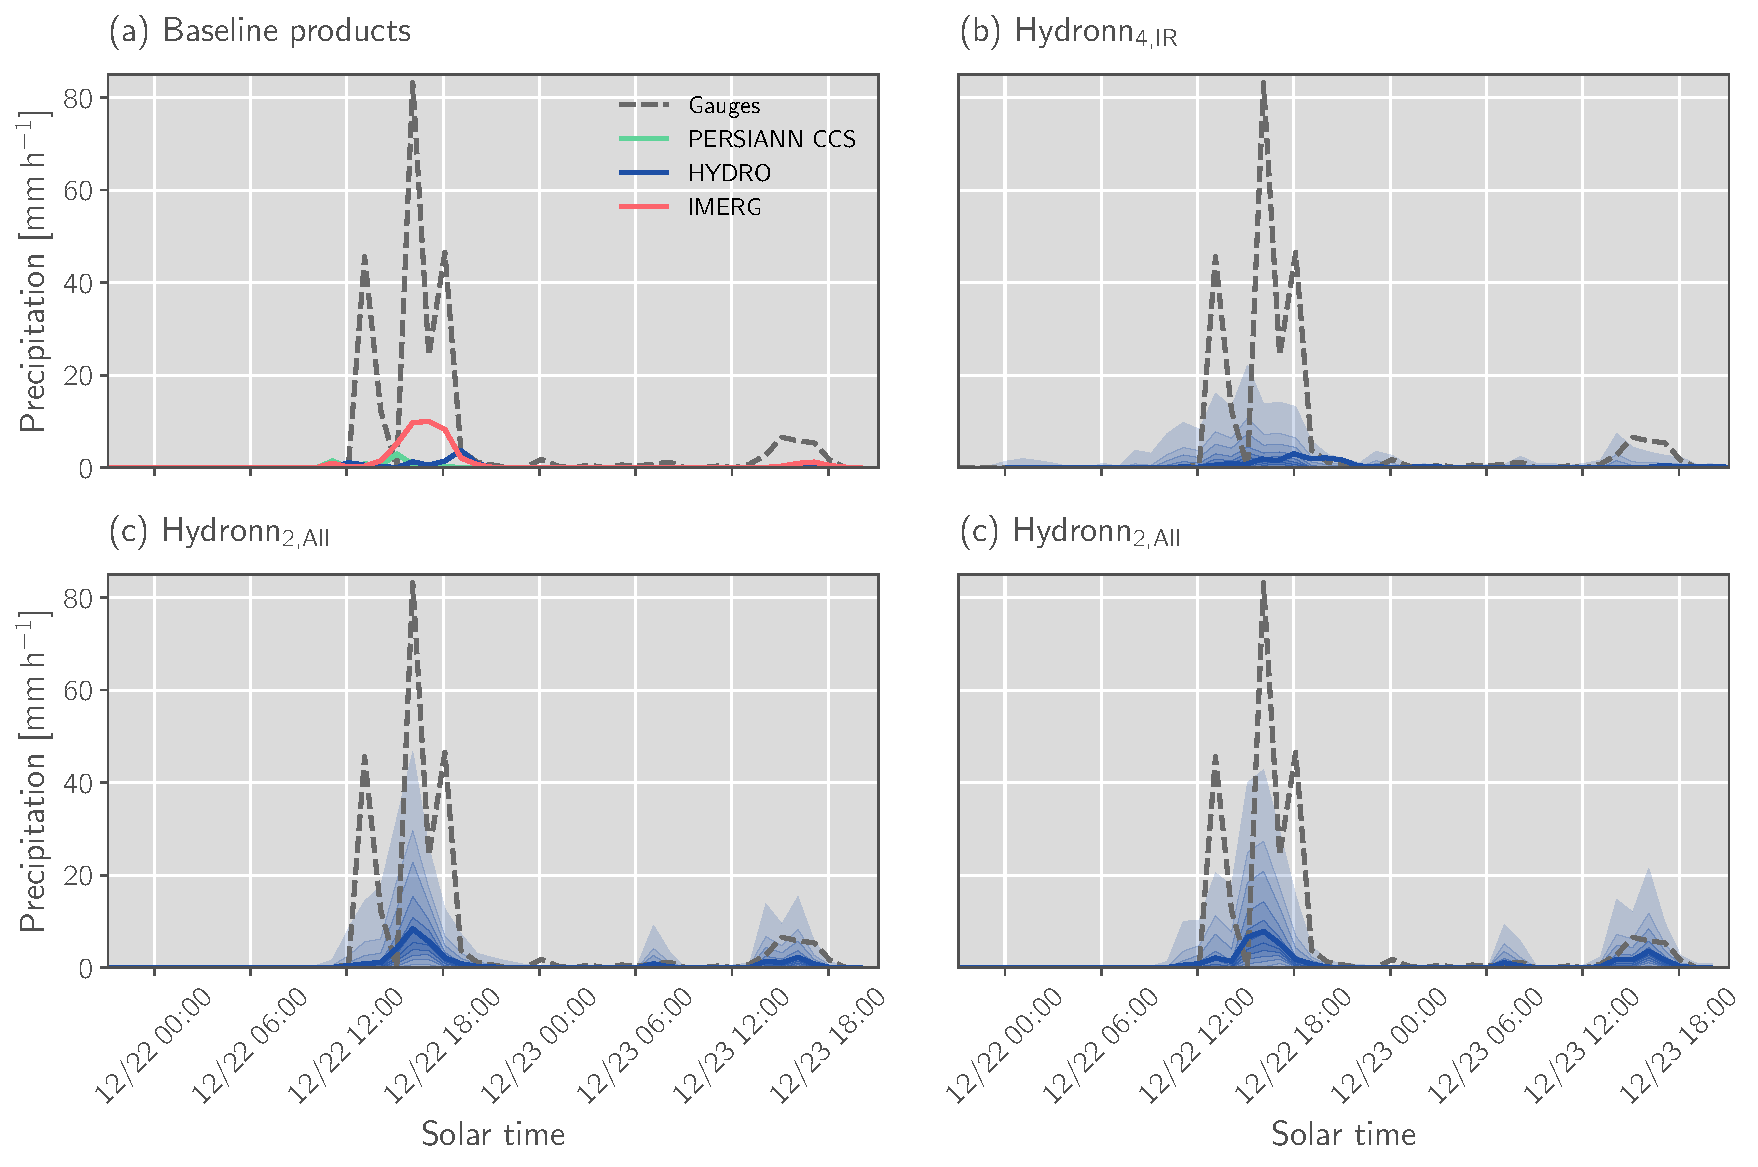
\includegraphics[width=\textwidth]{hydronn_case_study}
  \caption{
      Retrieved precipitation for a flood-producing precipitation even that
      occurred between 2020-12-22 and 2020-12-24 in the cite of Duque de Caxias
      in the state of Rio de Janeiro. Grey, dashed lines show the precipitation
      by the gauge station in Xer\'em. Solid lines show the retrieved mean
      precipitation for each retrieval algorithm. The shading shows filled
      contours of the posterior CDF at values $[0.01, 0.1, 0.2, \ldots, 0.8,
        0.9, 0.99]$.
    }
  \label{fig:contributions:hydronn_case_study}
\end{figure}

Besides a significantly improved near real-time retrieval for application over
Brazil, the principal results from this study are further proof of the ability
of neural-network-based retrievals to leverage the full potential of
latest-generation satellite imagery. The configuration that uses all available
channels at the highest possible resolution outperforms the GPM IMERG product,
which is one of the most advanced precipitation retrievals currently available
and integrates observations from a wide range of sensors and gauge measurements.

However, as can be seen in the results in
Fig.~\ref{fig:contributions:hydronn_case_study}, the retrievals from VIS and IR
observations still remain limited in their capabilities of detecting extreme
precipitation. While deep neural networks yield significant improvements in
retrieval performance, their instantaneous accuracy will always be limited by
the low information content of the observations. This suggest that future
retrieval development should try to further increase the amount of information
available to the retrieval, for example by incorporating the temporal evolution
of the observations or by merging observations from multiple sensors types.

\section{Cloud correction for data assimilation}

The final study included in this thesis is entitled
\textit{
  Can machine learning correct microwave humidity radiances for the influence of clouds?
  }
and published as \citet{kaur21} explores the application of QRNNs to remove the
effect of clouds from microwave observations. These observations contain
information on the temperature and distribution of water vapor in the atmosphere
and are used in data assimilation systems to find good initial conditions for
numerical weather forecasts. Since the assimilation usually involves simulating
the observations, the presence of hydrometeors in the atmosphere makes the
handling of observations that are affected by clouds much more complex. The
assimilation of both cloud-free and cloudy observations is referred to
as \textit{all-sky} assimilation. However, due to the complexity of handling the effects
of hydrometeors, less advanced assimilation systems discard cloudy observations
and only assimilate clear-sky observations.

This study investigates whether QRNNs can be used to detect and remove the
effect of clouds on microwave observations. If a model existed that could
accurately predict how cloudy-sky observations would look when the effect of
hydrometeors is removed, then this could, in principle, be used to handle these
observations in clear-sky assimilation systems. Since the ability to handle
cloud-affected observations significantly increases the number of observations
that can be ingested by the system, such a model could thus help to improve the
initialization of weather forecasts.

Because of their impact on the radiative transfer, operational data assimilation
systems have to detect observations affected by hydrometeors to either inflate
the uncertainties assigned to the observations (for all-sky assimilation) or
discard them altogether. Therefore, the first experiment in this study  assesses
the potential of applying QRNNs to predict a correction for cloud-contaminated
observations using an existing satellite sensor and compares the performance to
existing methods. The experiment shows that the QRNN-derived correction leads to
a lower bias in the observations than the residual biases in currently used
filtering methods, which reject up to $\SI{30}{\percent}$ of the observations.

The second experiment extended the approach to an upcoming satellite that will
be launched soon and a concept for a future satellite. Both of these satellites
will carry microwave sensors with channels above $\SI{300}{\giga \hertz}$. These
high frequencies make the observations more sensitive to scattering from ice
particles, which further complicates their use in data assimilation. In these
cases, using a QRNN-based cloud correction would provide a way to use the
additional information from the high-frequency channels to provide a more
accurate correction of lower frequency observations, which would improve the
impact of the lower frequency observations in the assimilation system. The
results show that observations at frequencies exceeding $\SI{300}{\giga \hertz}$
are well suited for cloud correction and thus demonstrate the potential of this
approach.

The principal result from this study is a proposed novel application of QRNNs
for the correction of microwave observations for use in data assimilation.
QRNN-based cloud correction provides superior performance to existing methods,
and the predicted uncertainties are more accurate than error estimates from
currently used error models. Moreover, the simulation-based assessment of the
potential of microwave observations at sub-millimeter wavelengths led to the
selection of these channels for an upcoming satellite mission
\citep{arctic_weather_satellite}.

\section{Future work}

The findings of this thesis suggest several directions of future research.
These will be discussed below.

\subsection{Handling retrieval uncertainty with neural networks}

This thesis has proposed and assessed neural-network-based methods for handling
uncertainties in remote sensing retrievals and shown their practicality across
multiple retrieval applications. The principal advantage of these methods is
certainly their simplicity. A minor modification in the training process is
required to migrate a deterministic neural network retrieval to a probabilistic
one. There are, however, two important limitations of the approaches: Their
incapability to handle correlations in the retrieval outputs and their reliance
on the aleatoric assumption, which postulates that the predictive uncertainty is
dominated by the aleatoric uncertainty.

It would therefore be valuable to systematically evaluate the approaches against
Bayesian neural networks and generative models on a set of atmospheric retrieval
problems. Such an evaluation should assess not only the retrieval accuracy but
also to take into account the effect on downstream applications of the data.
This would provide guidance in what scenarios the computationally more complex
alternative approaches should be applied.

\subsection{GPM precipitation retrievals}

Due to the good performance of the developed GPROF-NN retrievals, they are being
considered for the operational processing of the passive microwave retrievals of
the GPM mission. This will require additional investigations regarding the
climatological stability of the GPROF-NN retrievals across different satellites.

In addition to that, the migration to a neural-network-based implementation
opens up a number of opportunities for further improvements of the GPM passive
microwave retrievals. One of them is the extension of the training data to cover
multiple years of observations. It was found in \citep{pfreundschuh22d} that the
limited training period may be one reason for the retrieval errors on
climatological time scales. Besides that, including samples from the posterior
distribution may improve the representation of extreme precipitation in the
retrieval results, which is highly relevant for climate change studies.

\subsubsection{Novel retrieval applications}

As its name suggests, GPROF, the Goddard Profiling Algorithm, also retrieves
profiles of hydrometeors. These profiles consist comprise 28 vertical levels and
are retrieved at each pixel of the observations. However, because of storage
limitations, the profiles are compressed in the retrieval results, which causes
their accuracy to degrade.

One operational aspect of the GPROF-NN 3D retrieval that was discovered during
its development is that it does not require the ancillary data used by GPROF to
yield accurate. The ancillary provides information on the water content and
temperature of the atmosphere as well as the surface type to the retrieval.
Since these inputs need to be prepared, running the conventional GPROF retrieval
requires access to very specific datasets in addition to the satellite
observations.


Since the GPROF-NN 3D retrieval can be trained to work without the ancillary
data, it becomes much simpler to run the retrieval. It only requires access the
satellite observations, which can be readily downloaded from the internet, and
the neural network model, which has a non-compressed size of about
$\SI{250}{\mega \byte}$ and can thus also easily be distributed over the
internet. This opens up the possibility of providing users with uncompressed
retrieval results by giving them the opportunity to run the retrieval
themselves.

Since this lifts size constraints on the retrieval output, it provides a
practical way of developing and distributing a super-resolution retrieval for
the observations of the GMI microwave sensor. The spatial sampling of GMI is
$\SI{13.5}{\kilo \meter}$ in the along-track direction and $\SI{5}{\kilo
  \meter}$ in the across-track direction. The training data, which is derived
from the combined retrievals of the GPM core observatory, has a spatial sampling
of $\SI{5}{\kilo \meter} \times \SI{5}{\kilo \meter}$. Since the conventional
GPROF retrieval operates on single pixels, the training data is sub-sampled and
averaged to the footprint of the GMI pixels causing the high resolution of the
reference data to be lost. This, however, is not necessary for the CNN based
GPROF-NN retrieval. To explore the potential of performing super-resolution
retrievals, an experimental retrieval, named GPROF-NN HR, has been developed,
which retrieves precipitation at a three-times higher resolution in the
along-track direction of the GMI swath.

Very early results of such a retrieval are shown in
Fig.~\ref{fig:contributions:gprof_nn_hr}, which shows isosurfaces of retrieved
rain and snow water content as retrieved by GPROF and the three GPROF-NN
retrievals. The results for GPROF include the effects of the profile compression
that is applied to store them. The GRPOF-NN 1D and 3D retrievals yield clearly
better results, but the effects of the coarse along-track resolution are still
visible. The results of the GPROF-NN HR retrieval demonstrate its ability to
better resolve the rain bands in the hurricane. This suggests that the effective
resolution of the retrievals from GMI can be improved even further than what is
already achieved by the GPROF-NN retrievals.

%\begin{figure}
%  \centering
%  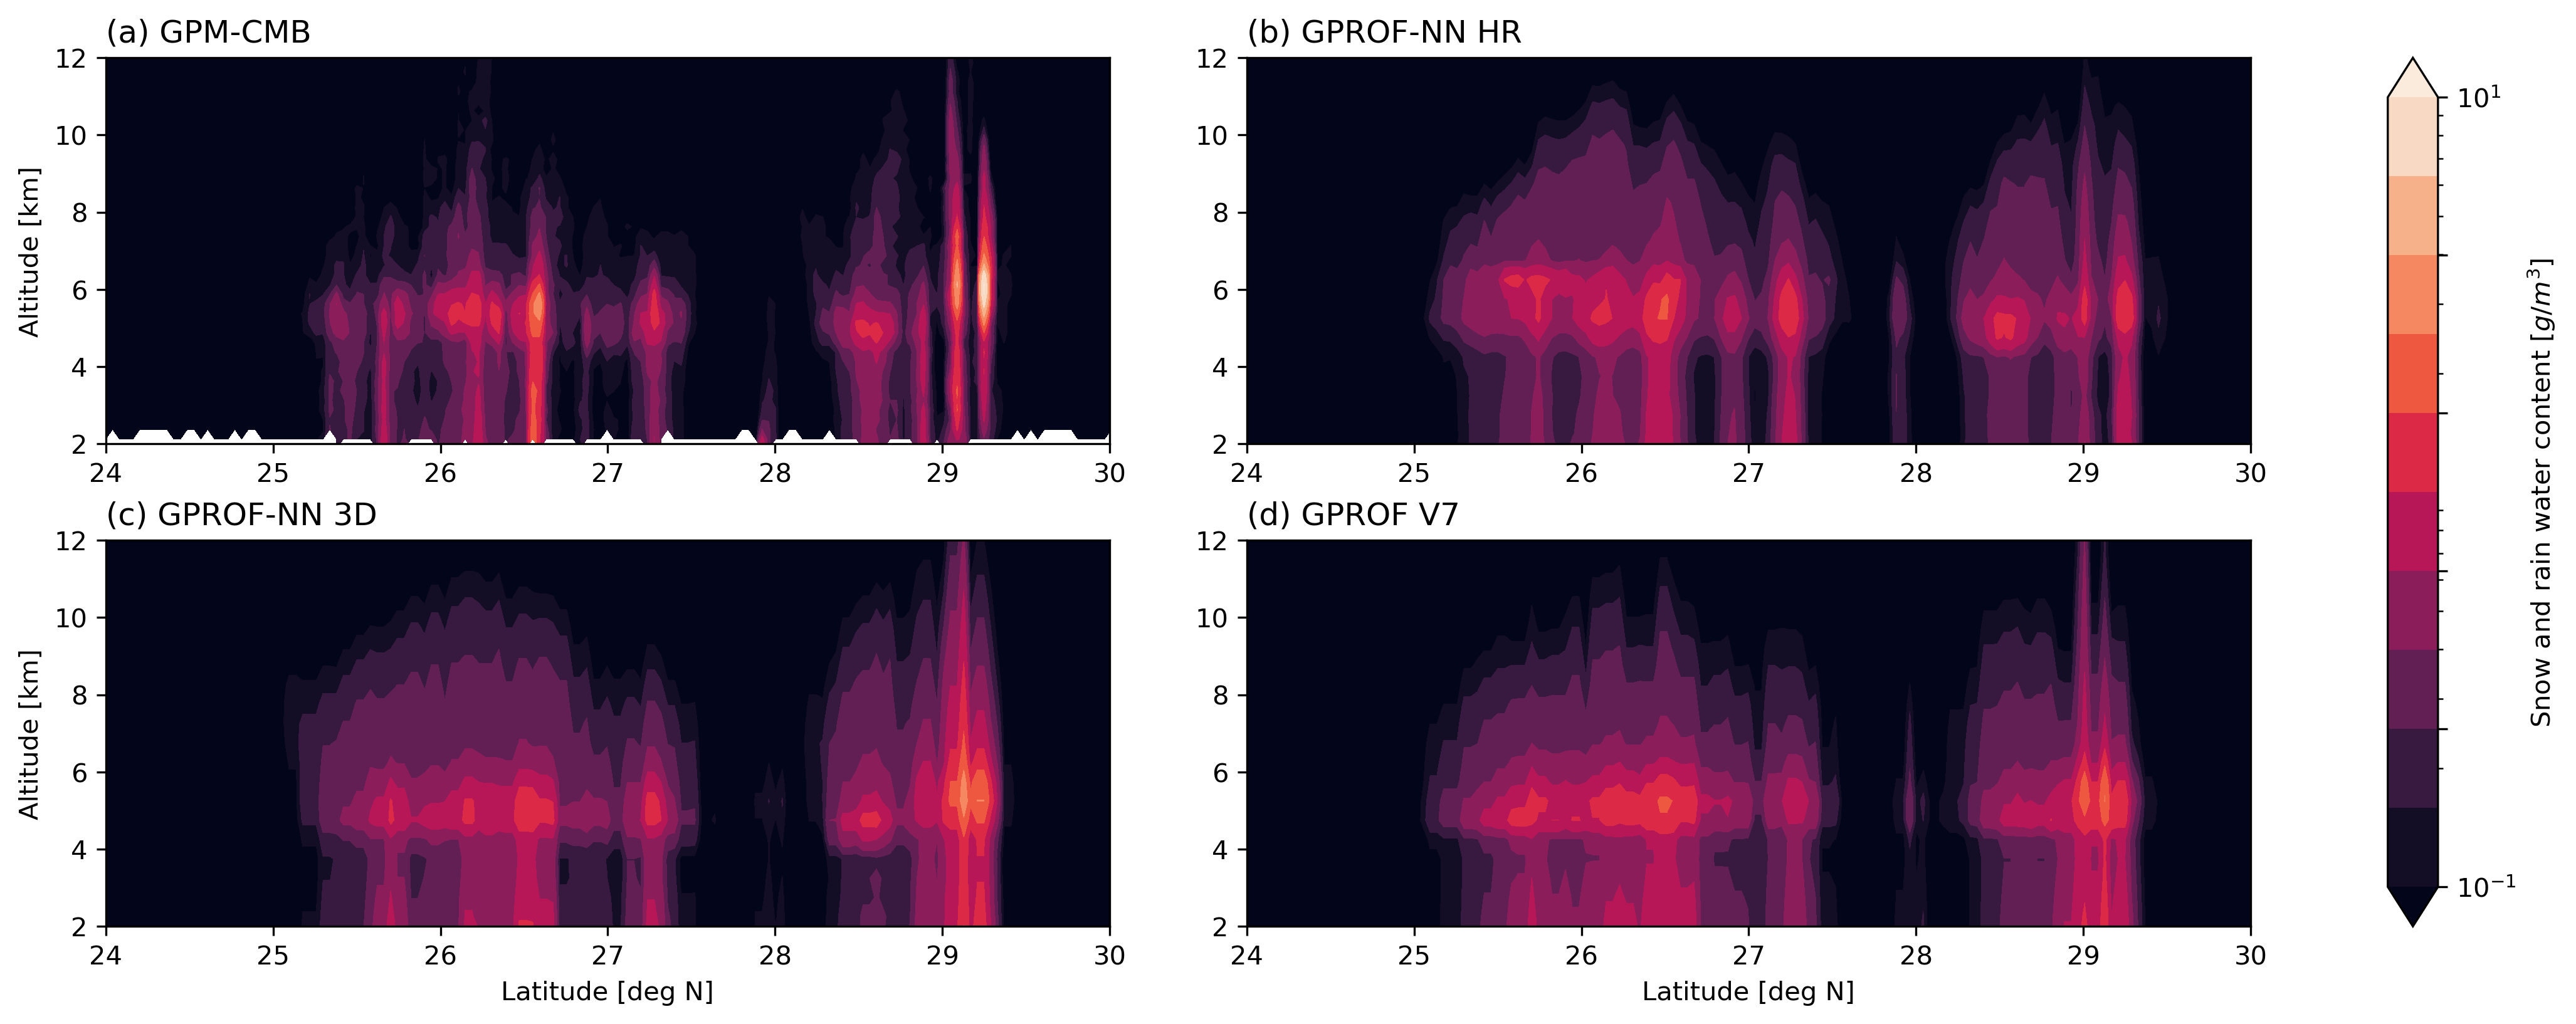
\includegraphics[width=\textwidth]{gprof_nn_hr}
%  \caption{Profiles of snow and rain water content in hurricane Ida. Each
%    panel shows retrieved precipitation profiles along the track of the
%    DPR on the GPM core observatory.
%  }
%  \label{fig:contributions:gprof_nn_hr}
%\end{figure}

\begin{figure}
  \centering
  \begin{subfigure}[b]{0.49\textwidth}
    \centering
    \includegraphics[width=\textwidth]{ida_gprof.0007}
    \caption{GPROF V7}
  \end{subfigure}
  \hfill
  \begin{subfigure}[b]{0.49\textwidth}
    \centering
    \includegraphics[width=\textwidth]{ida_gprof_nn_1d.0007}
    \caption{GPROF-NN 1D}
  \end{subfigure}
  \begin{subfigure}[b]{0.49\textwidth}
    \centering
    \includegraphics[width=\textwidth]{ida_gprof_nn_3d.0007}
    \caption{GPROF-NN 3D}
  \end{subfigure}
  \hfill
  \begin{subfigure}[b]{0.49\textwidth}
    \centering
    \includegraphics[width=\textwidth]{ida_gprof_hr.0007}
    \caption{GPROF-NN HR}
  \end{subfigure}
  \caption{
    Iso surfaces of rain water content (red) and snow water content (blue) in hurricane Ida
    shortly before landfall on 2021-08-29 15:14 UTC. For visualization purposes the
    vertical dimension is exaggerated by a factor of 10.
  }
  \label{fig:contributions:gprof_nn_hr}
\end{figure}


\subsection{Near real-time precipitation retrievals}

The results presented in \citet{pfreundschuh22b} clearly show the potential of
deep neural networks for precipitation retrievals from geostationary satellites.
According to personal communication, the developed retrieval is also being
considered for operational application.

An interesting result that emerged from this study was that, despite the low
information content of the geostationary observations on precipitation,
deep-learning-based retrievals can outperform highly complex retrieval pipelines
which integrate observations from multiple sensors. This indicates that the use
of information in current multi-sensor retrievals is sub-optimal. An upcoming
project will therefore explore the potential of directly fusing observations
from different sensors using a single neural network.


\bibliographystyle{plainnat}
\bibliography{references} 

\part{Appended papers}

\renewcommand{\chaptername}{Paper}
\setcounter{chapter}{0}

\chapter{A neural network approach to estimating a posteriori distributions of Bayesian retrieval problems} 
\chaptermark{Neural networks for Bayesian retrieval problems}            % Short title for the page header
\label{chap:qrnn}
\thispagestyle{empty}
\cleardoublepage            % skip back side of the page
\includepdf[pages=-]{papers/amt-11-4627-2018}

\chapter{GPROF-NN: A neural network based implementation of the Goddard Profiling Algorithm} 
\chaptermark{GPROF-NN}
\label{chap:qrnn}
\thispagestyle{empty}       % no page numbers
\cleardoublepage            % skip back side of the page
\includepdf[pages=-]{papers/gprof_nn_manuscript}

\chapter{An improved near-real time precipitation retrieval for Brazil} 
\chaptermark{Near-real time precipitation retrieval for Brazil}
\thispagestyle{empty}       % no page numbers
\cleardoublepage            % skip back side of the page
\includepdf[pages=-]{papers/manuscript}

\chapter{Can machine learning correct microwave humidity radiances for the influence of clouds?} 
\chaptermark{Correcting microwave humidity radiances for the influence of clouds}
\thispagestyle{empty}       % no page numbers
\cleardoublepage            % skip back side of the page
\includepdf[pages=-]{papers/amt-14-2957-2021}

\end{document}
